\documentclass[prb,twocolumn,amsmath,amssymb,floatfix]{revtex4-2}
\usepackage{graphicx}
\usepackage{bm}
\usepackage{placeins}
\usepackage[colorlinks=true,linkcolor=blue,citecolor=blue,urlcolor=blue]{hyperref}

\setcounter{topnumber}{3}\setcounter{bottomnumber}{2}\setcounter{totalnumber}{5}\setcounter{dbltopnumber}{2}
\renewcommand{\topfraction}{0.92}\renewcommand{\bottomfraction}{0.6}\renewcommand{\textfraction}{0.08}
\renewcommand{\floatpagefraction}{0.75}\renewcommand{\dbltopfraction}{0.92}\renewcommand{\dblfloatpagefraction}{0.75}
\newcommand{\Md}{M_{\rm dice}}
\newcommand{\eps}{\varepsilon}

\begin{document}

\title{Quantum order by disorder among lozenge tilings:\texorpdfstring{\\}{ }
a staircase of hub-free crystals between the Lieb ferrimagnet and the antiferromagnet}

\author{Suhwan Yoo}
\author{Jeehoon Choi}
\author{Chaeyeon Kim}
\author{Hee Young Kwon}
\author{Changyeon Won}
\email{cywon@khu.ac.kr}
\affiliation{Department of Physics, Kyung Hee University, Seoul 02447, Republic of Korea}

\date{\today}

\begin{abstract}
Lozenge tilings of the triangular lattice define an exponentially large family of bipartite networks, from the dice lattice, a Lieb ferrimagnet with the largest sublattice imbalance, to square-type tilings, which are compensated antiferromagnets. For the classical Heisenberg antiferromagnet all of them are degenerate. We show that quantum fluctuations lift this degeneracy through a local mechanism: to leading order the zero-point energy is a sum of single-site terms $\eps(z)$ that are convex in the coordination $z$, so that Jensen's inequality at fixed $\langle z\rangle=4$ selects the square-type tiling. A second-order expansion about the Ising limit gives this convexity analytically. A magnetic field, which couples to the Lieb moment, competes with the selection. Because the moment is carried most cheaply by threefold and fivefold sites, sixfold hubs are avoided, and we prove from the Lieb--Mattis theorem and bond counting that a hub-free tiling can carry at most $3/5$ of the dice moment. Combining sign-free quantum Monte Carlo for $S=\frac12$ to $\frac32$ with an enumeration of periodic tilings with up to 48 sites per cell (all but 22 of 403 cell shapes), we find that the competition produces a staircase of periodic crystals instead of a single jump. Its deepest and widest step is a hub-free crystal that saturates the bound, $M=\frac35\Md$, stable for $0.173J<h<0.268J$ at $S=\frac12$. Below it the hull is dense and shallow: crystals of threefold and fivefold defects, with the defects packed more closely at higher moment, lie within a few $10^{-4}J$ of one another, so that the magnetization rises in several narrow steps whose order is not resolved; their energies are described by a short-ranged lattice gas of curvature defects. Selection energies scale as $JS$, and for $S=\frac12$ to $\frac32$ the field at which a hub-free crystal gives way to dice changes by less than 12\% in units of $J$. In the height representation $z$ measures the discrete Gaussian curvature and the Lieb moment the sublattice-staggered curvature, and the $\frac35\Md$ crystal is the densest packing of sublattice-sorted $\pm\pi/2$ cones and saddles. We give spectroscopic signatures of each crystal and discuss realizations in nanographenes, atomic spin arrays and quantum simulators.
\end{abstract}

\maketitle

\begin{figure*}[t]
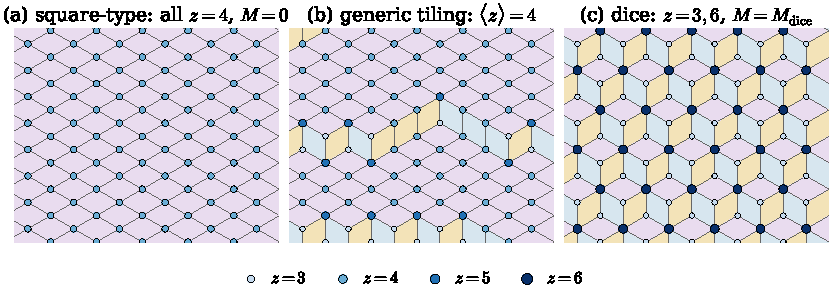
\includegraphics[width=0.9\textwidth]{figs/fig1_tilings.pdf}
\caption{Lozenge tilings of the triangular lattice and the bipartite networks they define. Rhombi are shaded by orientation, and sites are colored and sized by coordination $z$. (a)~Square-type tiling: all $z=4$, compensated ($M=0$). (b)~A generic tiling, with $z$ varying from site to site; every tiling has $\langle z\rangle=4$. (c)~Dice lattice: sixfold hubs and threefold rims, Lieb moment $\Md=SN/3$. All tilings have the same classical energy $-2JS^2N$.}
\label{fig:tilings}
\end{figure*}

%=====================================================================
\section{Introduction}
%=====================================================================

Order by disorder is the selection of a subset of classically degenerate ground states by fluctuations~\cite{Villain1980,Henley1989}. In frustrated magnets the degenerate manifold is usually a family of spin configurations on a \emph{fixed} lattice. Thermal or quantum fluctuations then pick the configurations with the softest excitation spectrum, most often collinear or coplanar ones. Harmonic zero-point energies then often reduce to local effective Hamiltonians on the degenerate manifold~\cite{Henley2006}. In this paper we study a different kind of degeneracy, one in which the object that is degenerate is the \emph{lattice itself}. The tilings below are fixed exchange graphs, each with its own Hamiltonian. Comparing their ground-state energies selects a lattice when the graph can rearrange while the spins stay in their ground state, i.e., when the tiling is an annealed degree of freedom. This is the situation in growth, self-assembly and programmable arrays, in which the network is a design or growth variable (Sec.~\ref{sec:disc}). We use ``order by disorder'' in this sense: quantum fluctuations select the graph.

Consider the lozenge (rhombus) tilings of the triangular lattice. Each tiling is obtained by pairing every up triangle with one of its down neighbors into a rhombus and deleting the shared edge. The remaining bonds form a planar bipartite graph in which every site has coordination $3\le z\le6$ and the mean coordination is exactly $\langle z\rangle=4$ [Fig.~\ref{fig:tilings}]. Two extreme members of this family are familiar. The dice ($\mathcal{T}_3$) lattice~\cite{Sutherland1986,Vidal1998} has sixfold hubs and threefold rims. The square-type tiling has only fourfold sites and is topologically the square lattice. By the Lieb--Mattis theorem~\cite{LiebMattis1962,Lieb1989}, the Heisenberg antiferromagnet on any of these graphs has a ground state with total spin $S_{\rm tot}=S|N_A-N_B|$. The dice lattice is therefore a ferrimagnet with the largest possible moment $\Md=SN/3$, while the square-type tiling is compensated. The family thus spans ferrimagnets and antiferromagnets continuously.

For classical spins every tiling has the same energy, $E_{\rm cl}=-JS^2N_b=-2JS^2N$, because every tiling has $N_b=2N$ bonds and collinear N\'eel order satisfies all of them. The number of tilings grows exponentially with $N$. Quantum mechanically the degeneracy is lifted, and two natural questions follow. Which lattice do quantum fluctuations select, and why? And how does a magnetic field, which couples directly to the Lieb moment and therefore favors the dice tiling, compete with that selection?

Quantum antiferromagnets on quasiperiodic and dice-derived networks have been studied by Jagannathan, Wessel and co-workers~\cite{Wessel2003,Jagannathan2006,Szallas2009,Jagannathan2012,Jagannathan2013}. Two of their results bear directly on the questions above. On the Penrose tiling, phason disorder lowers the ground-state energy~\cite{Szallas2009}. On the staggered dice lattice (SDL), a lozenge tiling with coordinations $z=3,4,5$ in equal numbers and $N_A=N_B$, local ``phason flips'' that create $z=3$ and $z=6$ sites raise it and enhance the staggered moment~\cite{Jagannathan2012}; domain walls between phason domains carry a positive line energy ($\approx0.062J/a$) and feel a Casimir-like $1/d$ interaction~\cite{Jagannathan2013}. The authors described the enhancement of the staggered moment by geometric disorder as ``order by disorder''; we use the term for the selection of the graph itself. The two energy results have opposite signs. Section~\ref{sec:zero} shows that the SDL result follows from a convex site energy of the coordination, and that the Penrose result is consistent with it if disorder narrows the distribution of coordinations. These studies kept the two sublattices balanced, considered random or dilute flips, and did not include a field. The questions posed above involve sectors with different sublattice imbalance, systematic control of that imbalance, and the competition with a Zeeman field. To our knowledge they have not been addressed.

Our main results are as follows.
(i) The zero-point energy of any tiling is accurately a sum of single-site energies $\eps(z)$, and $\eps(z)$ is convex. Jensen's inequality therefore selects uniform $z=4$ tilings, which as graphs are all square lattices, at zero field. The resulting selection energy is $\propto JS$ and can be computed for any tiling by counting coordinations [Fig.~\ref{fig:mech}].
(ii) Domain walls between dice and square regions have \emph{negative} energy, $\sigma\approx-0.013J/a$ [Fig.~\ref{fig:tilt}]. The field-driven crossover is therefore not a single first-order jump through phase coexistence.
(iii)~A second-order expansion about the Ising limit gives the selection energy as a sum over bonds of a convex function of $z_i+z_j$. It reproduces the convexity, the shape of the energy hull and the signs of the defect interactions without fit parameters.
(iv)~A tiling without sixfold hubs carries at most $\frac35\Md$. This bound follows from the Lieb--Mattis theorem and bond counting and is saturated only when every minority-sublattice site has $z=5$.
(v)~The crossover is a magnetization staircase of periodic crystals, established by enumeration of periodic tilings with up to 48 sites per cell and quantum Monte Carlo (QMC) [Figs.~\ref{fig:crystals} and~\ref{fig:stair}, Table~\ref{tab:crystals}]. Its deepest and widest step is a crystal that saturates the hub-free bound. Below it the steps are dense and narrow; the crystals are successive packing stages of $z=3$ and $z=5$ defects, governed by a short-ranged interaction in which like-sign curvature attracts [Fig.~\ref{fig:gas}].
(vi)~Each plateau carries distinct fluctuation, entanglement and dynamical signatures [Figs.~\ref{fig:fluct} and~\ref{fig:sqw}], and selection energies scale as $JS$, so that step fields expressed in $J$ depend only weakly on $S$ [Fig.~\ref{fig:spinS}].
(vii)~In the height representation, $z$ is exactly the discrete Gaussian curvature of a lifted surface, and the Lieb moment is its sublattice-staggered total, so that zero field selects folded, curvature-free surfaces and the field crumples them with conical defects (Appendix~\ref{app:geom}). In an effective tiling model the $\Md/2$ crystal melts at $T\simeq0.02$--$0.03J$, and local-flip dynamics become trapped on cooling (Appendix~\ref{app:finiteT}).

The paper is organized as follows. Section~\ref{sec:model} defines the model and its classical degeneracy, and Sec.~\ref{sec:methods} summarizes the methods. Section~\ref{sec:zero} explains the zero-field selection, its origin in the Ising limit and the hub-free bound. Section~\ref{sec:field} presents the field-driven crystals and the staircase. Sections~\ref{sec:fluct} and~\ref{sec:spinS} discuss fluctuations and the dependence on $S$. Section~\ref{sec:disc} discusses interpretation, platforms and limitations, and Sec.~\ref{sec:concl} concludes. The appendices give the geometric interpretation, tests of the models, finite-size effects and the finite-temperature behavior of an effective tiling model.

%=====================================================================
\section{Model and classical degeneracy}\label{sec:model}
%=====================================================================


We consider
\begin{equation}
H_{\mathcal T}=J\sum_{\langle ij\rangle\in\mathcal T}\mathbf S_i\cdot\mathbf S_j-h\sum_iS_i^z,\qquad J>0,
\label{eq:H}
\end{equation}
where the sum runs over the bonds of a lozenge tiling $\mathcal T$ of an $L\times L$ triangular torus ($N=L^2$ sites) with primitive vectors $\mathbf a_1$ and $\mathbf a_2$ at $60^\circ$. Each tiling is specified by a perfect matching of up and down triangles, which is equivalent to a dimer covering of the honeycomb lattice. Its height function~\cite{BloteHilhorst1982,Kenyon2006} has an average slope (tilt) that is conserved by the elementary hexagon flip, i.e., the rotation of three rhombi around a site with $z=3$. The tilt therefore labels topological sectors on the torus.

Every tiling has $2N$ bonds, so $\langle z\rangle=4$. The graph is bipartite with sublattices $A$ and $B$. By the Lieb--Mattis theorem~\cite{LiebMattis1962,Lieb1989} the ground state has $S_{\rm tot}=S|N_A-N_B|\equiv M$. We write $m=|N_A-N_B|/(2N)$ for the imbalance per site, so that $m=1/6$ for dice. The imbalance is not a topological invariant, since a single hexagon flip changes $N_A-N_B$ by 2. However, strips of dice and square-type tiling separated by straight walls provide a systematic family that interpolates between $m=0$ and $m=1/6$. We call it the ``tilt family'' below.

Classically, every tiling admits a collinear N\'eel state with energy $-JS^2$ per bond, so all tilings are degenerate at $h=0$. For $h>0$ the dice tiling wins immediately through its Zeeman energy $-hM$. The classical magnetization therefore jumps from 0 to $\Md$ at $h=0^+$ [dashed line in Fig.~\ref{fig:stair}(b)]. Everything that follows is a quantum effect.

%=====================================================================
\section{Methods}\label{sec:methods}
%=====================================================================

\emph{Quantum Monte Carlo.} All tilings considered here are bipartite, so Eq.~(\ref{eq:H}) is sign-free. We use the stochastic series expansion (SSE)~\cite{Sandvik1999} with directed loops~\cite{Syljuasen2002} and heat-bath exit probabilities, for general $S$ and with the field included in the bond operators. The code was checked against exact diagonalization (ED) of 27-site tori for $S=\frac12,1,\frac32$. We use $\beta J=L$ for $S=\frac12$ ($L=12$--$36$), $\beta J=36$ for the cell clusters below, and $\beta JS=12$ for the spin-$S$ runs at $L=12$. We did not extrapolate in $\beta$. In such a field the ferrimagnetic crystals are gapped, by $h$ for the former Goldstone mode and by $\Delta_+-h$ for the moment-raising branch (Sec.~\ref{sec:fluct}), At the fields used ($h=0.07$--$0.24J$, below $\Delta_+$ of each crystal) both gaps are at least $0.05J$, so that $e^{-\beta\Delta}\lesssim0.17$. A systematic $\beta$ extrapolation, which would quantify the remaining thermal contribution of the low-lying magnon band, is left for future work. The zero-field energy of a tiling is obtained from a run at a field $h$ below its moment-raising gap $\Delta_+$ as $e_0=e+hm_{\rm meas}$, where $e$ is the measured energy per site including the Zeeman term. For ferrimagnetic crystals $m_{\rm meas}$ equals the Lieb value $m$ to within $10^{-4}$ in every run, because the ground-state multiplet is pinned at $S^z_{\rm tot}=M$, so this subtraction is exact up to that accuracy. For the compensated square-type tiling we use $e_0=e+\frac12\chi h^2$ with $\chi\simeq0.065J^{-1}$ per site, from our own runs at $L=24$ ($m/h=0.064$--$0.070$ for $h=0.1$--$0.2J$). Our square-type energy at $L=24$, $e_0=-0.66917(30)J$, lies $3\times10^{-4}J$ above the thermodynamic-limit value~\cite{Sandvik1997}, whereas finite-size LSWT predicts a value $1.5\times10^{-4}J$ below it. We attribute the difference of about $4.5\times10^{-4}J$ mainly to the finite $\beta J=24$. Because the compensated reference enters only the first step, an offset of this size would shift the onset field (by up to $0.03J$ at $\frac1{11}\Md$) but none of the steps between ferrimagnetic crystals. As a graph the square-type tiling \emph{is} the square lattice, so we use the thermodynamic-limit value $e_{\rm sq}=-0.669437(5)J$ of Ref.~\cite{Sandvik1997} as the zero-moment reference. This matters because finite-size corrections differ between compensated and ferrimagnetic tilings. In linear spin-wave theory (LSWT) the energy per site of the compensated square-type tiling on an $L\times L$ torus deviates from the thermodynamic limit by $-1.2\times10^{-3}$, $-1.5\times10^{-4}$ and $-4\times10^{-5}J$ at $L=12$, $24$ and $36$, whereas for the ferrimagnetic crystals the deviation is below $5\times10^{-6}J$ at $L=36$ (e.g., $-4\times10^{-8}J$ for $\Md/2$). In particular, a size-dependent term proportional to the total moment, $\alpha|\mu|/N$ with $\mu=(N_A-N_B)/2$, which appears when a few uncompensated defects sit in a compensated background, is absent for crystals with an extensive moment. We therefore compare crystals at $L=36$ with the thermodynamic square-lattice reference. Crystals whose cells do not fit an $L\times L$ torus are simulated on $k\times k$ copies of their cell, with periodic boundary conditions along $k\mathbf v_1$ and $k\mathbf v_2$ and $N=825$--$1280$ ($\beta J=36$); for these extensive-moment crystals the LSWT energy of such clusters agrees with the thermodynamic limit to $4\times10^{-5}J$ or better.

\emph{Spin-wave theory on arbitrary graphs.} For a bipartite graph with adjacency matrix $A$ and degree matrix $D$, LSWT gives magnon energies $\omega_\nu=JS|\lambda_\nu|$, where $\lambda_\nu$ are the eigenvalues of $\mathcal L^{1/2}P\mathcal L^{1/2}$, with $\mathcal L=D-A$ the graph Laplacian and $P={\rm diag}(\eta_i)$ the sublattice signs ($\eta_i=\pm1$). It also gives the ground-state energy $E=-JS^2N_b+\frac{JS}2(\sum_\nu|\lambda_\nu|-\sum_iz_i)$. We diagonalize the full bosonic Hamiltonian with Colpa's method~\cite{Colpa1978} to obtain spin deviations, Gaussian entanglement entropies and $S^{xx}(\mathbf q,\omega)$. Zero modes ($\omega<10^{-2}J$) are excluded.

\emph{Search over tilings.} We use three complementary searches. (a)~\emph{Periodic enumeration:} for supercells $\mathbf v_1=(p,0)$, $\mathbf v_2=(s,q)$ with $pq\le48$, we enumerate all tilings (up to $2\times10^7$ per cell) and keep the bipartite ones (on a torus some tilings are not bipartite). We group them into structural classes by a translation-invariant fingerprint (the coordination histogram together with the multiset of neighbor coordinations) and keep one representative per class, retaining every class within $0.03J$ of the coordination-model minimum at each $m$, so that tilings with the same coordination histogram but different arrangements are kept. Candidates within $2$--$3\times10^{-3}J$ of the coordination-model minimum (Sec.~\ref{sec:zero}) at each $m$, and every hub-free class for $pq\le36$, are evaluated with LSWT in the thermodynamic limit, and the hull structures with QMC. Supercells related by the point group $D_6$ are treated once (Sec.~\ref{sec:field}). (b)~\emph{Annealing:} simulated annealing in tiling space with local flips is performed at fixed tilt for $L=18,24,30$, first with the coordination model and then with the full LSWT energy. This produces the irregular networks shown in gray in Fig.~\ref{fig:stair}(a). (c)~\emph{Tilt family:} strips of dice and square tiling, used to extract wall energies.

%=====================================================================
\section{Zero field: why the square-type tiling wins}\label{sec:zero}
%=====================================================================

\begin{figure}[t]
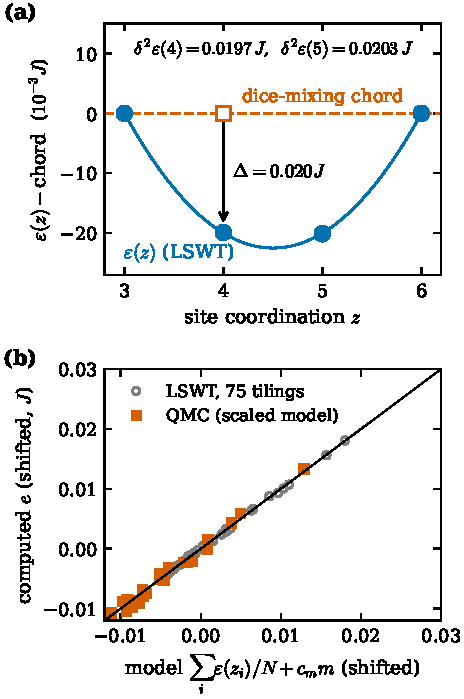
\includegraphics[width=\columnwidth]{figs/fig2_mechanism.pdf}
\caption{Coordination mechanism of quantum tiling selection ($S=\frac12$). (a)~Single-site zero-point energies $\eps(z)$ obtained by fitting LSWT energies of 75 tilings to Eq.~(\ref{eq:coord}), plotted relative to the chord joining $z=3$ and $z=6$ (dashed; the dice composition). The large linear trend of $\eps(z)$ is removed, so its convexity appears as the dip below the chord. The discrete second differences $\delta^2\eps(z)=\eps(z+1)+\eps(z-1)-2\eps(z)$ are $0.0197J$ ($z=4$) and $0.0203J$ ($z=5$). At fixed $\langle z\rangle=4$ the uniform $z=4$ tiling therefore lies below the dice combination (open square) by $\Delta=0.020J$ per site. (b)~Energies computed for many tilings vs the coordination model: LSWT (open circles, rms residual $1.4\times10^{-4}J$) and QMC with the model rescaled linearly, $e_{\rm QMC}=c_0+c_1e_{\rm model}$, with the two parameters $c_0$ and $c_1$ fitted to these data (squares, rms $5\times10^{-4}$--$8\times10^{-4}J$). Both axes are shifted by a common constant.}
\label{fig:mech}
\end{figure}

\subsection{A local, convex zero-point energy}\label{sec:local}

We first computed the LSWT energy of 75 tilings with widely different structure: tilt-family strips, and tilings with up to 200 random flips. Their energies are reproduced by a purely local form,
\begin{equation}
\frac{E_{\rm LSWT}}{N}\simeq\frac1N\sum_i\eps(z_i)+c_m\,m ,
\label{eq:coord}
\end{equation}
with
\begin{equation*}
\eps(3,4,5,6)=(-0.8544,\,-0.6582,\,-0.4423,\,-0.2061)J
\end{equation*}
and $c_m=0.0304J$ for $S=\frac12$. Because $\sum_i(z_i-4)=0$ for every tiling, $\eps(z)$ is defined only up to a term $\lambda(z-4)$, which changes no energy; the values above are the minimum-norm least-squares solution. Only $\eps(4)$ and combinations that are invariant under this shift, such as the second differences and the costs of neutral groups below, are physical. The rms residual is $1.4\times10^{-4}J$, compared with a spread of energies of $6.8\times10^{-3}J$ [Fig.~\ref{fig:mech}(b)]. The small $c_m$ term accounts for the weak cost of sublattice imbalance.

The key property is that $\eps(z)$ is \emph{convex} [Fig.~\ref{fig:mech}(a)], a statement that is invariant under the shift above. Physically, the zero-point energy gained by spreading quantum fluctuations over more bonds saturates as $z$ grows, so replacing two $z=4$ sites by a $z=3$ and a $z=5$ site costs energy. Because $\sum_iz_i=4N$ is fixed for every tiling, Jensen's inequality gives
\begin{equation}
\frac1N\sum_i\eps(z_i)\;\ge\;\eps(\langle z\rangle)=\eps(4),
\label{eq:jensen}
\end{equation}
with equality only when all $z_i=4$. Every other tiling pays for its coordination variance. Tilings with all $z_i=4$ are not unique: besides the square-type tiling there are folded variants (Appendix~\ref{app:geom}). As graphs, however, all of them are square lattices, so the zero-field ground state is in every case the square-lattice antiferromagnet. The dice lattice, whose coordinations $3,3,6$ lie farthest from 4, is the most expensive at $h=0$. The same inequality gives the sign found in Ref.~\cite{Jagannathan2012}: flips in the SDL create $z=3$ and $z=6$ sites from $z=4$ and $z=5$ sites, which widens the coordination distribution and raises the energy. On the Penrose tiling, where phason disorder lowers the energy~\cite{Szallas2009}, the convex picture requires that disorder narrow the distribution of coordinations; we have not checked this.

\emph{How good is the local model?} We tested Eq.~(\ref{eq:coord}) in four ways (Appendix~\ref{app:tests}). (i)~On an enlarged training set of 128 tilings ($L=18,24$, up to 600 random flips) the rms residual is $1.6\times10^{-4}J$ in leave-one-out cross-validation, with no systematic dependence on system size, number of flips or starting structure (largest class-averaged residual $1.8\times10^{-4}J$). (ii)~Adding the number of bonds of each type $(z_i,z_j)$ as extra terms halves the residual, to $0.9\times10^{-4}J$. Correlations between neighboring coordinations are therefore present but small. (iii)~Out of sample, on 71 periodic crystals evaluated with LSWT in the thermodynamic limit, the residual is $2.4\times10^{-4}J$ ($1.5\times10^{-4}J$ with pair terms). (iv)~Tilings with \emph{identical} coordination histograms but different arrangements differ by at most $3.5\times10^{-4}J$; these arrangement energies are described in Sec.~\ref{sec:gas}. The model therefore resolves differences of order $10^{-3}J$, such as the depth of the $\frac35\Md$ hull point, but not differences of order $10^{-4}J$. We use it only to screen candidates. Every energy on which a conclusion rests is computed with QMC.

QMC confirms this picture quantitatively. For $S=\frac12$ the square-type tiling has $e_0=-0.669437(5)J$~\cite{Sandvik1997} and the dice tiling $-0.63786(30)J$, a difference of $0.0316J$ per site, compared with zero classically. The QMC energies of all structures studied, including strips, periodic crystals and annealed networks, follow the coordination model after a single linear rescaling, $e_{\rm QMC}=c_0+c_1\,e_{\rm model}$ with $c_1=1.27$, to $5$--$8\times10^{-4}J$ [Fig.~\ref{fig:mech}(b)]. This model is what makes the exhaustive searches of Sec.~\ref{sec:field} possible.

\subsection{Origin of the convexity: expansion about the Ising limit}\label{sec:ising}

The convexity of $\eps(z)$ can be derived. Split $H_{\mathcal T}$ at $h=0$ into $H_{zz}=J\sum S^z_iS^z_j$ and $H_\perp=\frac J2\sum(S^+_iS^-_j+{\rm h.c.})$, and treat $H_\perp$ as a perturbation of the N\'eel state, which is a ground state of $H_{zz}$ on every bipartite tiling. $H_\perp$ acts on one bond at a time: it lowers the spin at one end of $\langle ij\rangle$ and raises it at the other, with matrix element $JS$. This costs $J[S(z_i+z_j)-1]$, because each of the other $z_i-1$ and $z_j-1$ bonds at $i$ and $j$ loses $JS$ and the bond itself loses $J(2S-1)$. To second order the energy per site is
\begin{equation}
e=-\frac{JS^2N_b}{N}-\frac{JS}{N}\sum_{\langle ij\rangle}\frac1{z_i+z_j-1/S}.
\label{eq:ising}
\end{equation}
Equation~(\ref{eq:ising}) has no adjustable parameter. It scales as $JS$, as the full selection energy does (Sec.~\ref{sec:spinS}), and it contains the qualitative content of this section and the next.

(1)~\emph{Convex site energies.} For defects that do not touch, every bond of a site with coordination $z$ has a $z=4$ partner. Using $\sum_i(z_i-4)=0$, Eq.~(\ref{eq:ising}) then reduces to the site form of Eq.~(\ref{eq:coord}) with
\begin{equation}
\eps(z)=-JS\,\frac{z}{z+4-1/S}+\lambda(z-4)+{\rm const}.
\label{eq:epsI}
\end{equation}
The fraction $z/(z+c)$ is concave, so $\eps(z)$ is convex. Physically, a site with more bonds has more channels for quantum fluctuations, but each fluctuation frustrates more bonds and costs more energy. The gain therefore saturates with $z$. For $S=\frac12$ the second differences are $\delta^2\eps(4)=0.0095J$ and $\delta^2\eps(5)=0.0060J$, compared with $0.020J$ from LSWT. A pair of a $z=3$ and a $z=5$ site costs $0.0048J$ per unit of moment charge (defined below), and a hub with two $z=3$ sites costs $0.0063J$, 31\% more.

(2)~\emph{Contact energies.} When two defects share a bond, the bond term of Eq.~(\ref{eq:ising}) no longer separates into site terms. Replacing a $(3,4)$ and a $(4,5)$ bond by a $(3,5)$ and a $(4,4)$ bond costs $\frac J2(\frac15+\frac17-\frac13)=+4.8\times10^{-3}J$ for $S=\frac12$, so bonded defects of opposite curvature repel. Bonded like defects, $(3,3)$ and $(5,5)$, attract, by $-8.3$ and $-3.0\times10^{-3}J$. The lattice-gas fit to LSWT in Sec.~\ref{sec:gas} gives $+4.39$ and $-3.24\times10^{-3}J$ for the same contacts.

(3)~\emph{Shape of the hull.} Relative to its own straight line between the square-type and dice tilings, Eq.~(\ref{eq:ising}) gives deviations of $-1.6$, $-1.9$, $-2.3$, $-2.4$, $-2.9$, $-3.2$, $-3.7$, $-4.4$, $-4.8$ and $-4.0\times10^{-3}J$ for the crystals at $M/\Md=\frac1{11},\frac19,\frac17,\frac16,\frac15,\frac14,\frac13,\frac12,\frac35$ and $\frac23$ of Sec.~\ref{sec:field}. The QMC values are $-2.4$, $-2.7$, $-2.9$, $-3.1$, $-3.5$, $-4.0$, $-4.5$, $-5.0$, $-5.3$ and $-4.4\times10^{-3}J$. In particular, Eq.~(\ref{eq:ising}) places the minimum at the hub-free $\frac35\Md$ crystal. It underestimates the overall scale: $e_{\rm dice}-e_{\rm sq}=0.0238J$, compared with $0.0316J$ in QMC. Equation~(\ref{eq:ising}) is therefore a qualitative guide. All conclusions below rest on LSWT and QMC.



\subsection{The cost of a moment: why hubs are avoided, and a bound}\label{sec:cost}

Equation~(\ref{eq:coord}) also tells us how a tiling can acquire a moment most cheaply. On any bipartite tiling each bond joins $A$ to $B$, so $\sum_{i\in A}z_i=\sum_{i\in B}z_i=2N$. Writing $q_i=\pm(z_i-4)$, with $+$ on the minority sublattice $A$ and $-$ on $B$, this gives
\begin{equation}
m=\frac{N_B-N_A}{2N}=\frac1{8N}\sum_i q_i .
\label{eq:charge}
\end{equation}
Every site with $z\ne4$ thus carries a ``moment charge'' $q_i$. Because $\sum_i(z_i-4)=0$, charges come in neutral groups, and only the cost of a neutral group is defined unambiguously. The cheapest group is a $z=5$ site on $A$ with a $z=3$ site on $B$: charge $+2$ at cost $\eps(5)+\eps(3)-2\eps(4)=0.0197J$, i.e., $0.0099J$ per unit charge. A hub requires a $z=6$ site on $A$ and two $z=3$ sites on $B$: charge $+4$ at cost $\eps(6)+2\eps(3)-3\eps(4)=0.0597J$, i.e., $0.0149J$ per unit charge, 50\% more. To leading order, the energy therefore rises \emph{linearly} with $m$, with slope $8\times0.0099J+c_m\approx0.11J$, as long as the moment can be carried by aligned $3/5$ pairs alone. It rises more steeply once hubs become unavoidable.

The largest moment that $3/5$ pairs can carry follows from bond counting. Let a tiling contain no hubs, so that $z_i\le5$ for every site. Then $2N=\sum_{i\in A}z_i\le5N_A$, i.e., $N_A\ge\frac25N$, and with $N_A+N_B=N$
\begin{equation}
m=\frac{N_B-N_A}{2N}\le\frac1{10},\qquad M\le\tfrac35\,\Md .
\label{eq:bound}
\end{equation}
By the Lieb--Mattis theorem this is a bound on the ground-state spin of every hub-free tiling. Equality requires $z_i=5$ on every site of $A$. The $B$ sites then have $\sum_{i\in B}z_i=2N$ on $N_B=\frac35N$ sites, i.e., $\langle z\rangle_B=\frac{10}3$, and $B$ sites may in principle have $z=3$, 4 or 5. The leading-order energy, Eq.~(\ref{eq:coord}), selects among these histograms. If $B$ carries only $z=3$ and $z=4$, two thirds of its sites have $z=3$ and one third $z=4$, i.e., $z_3{:}z_4{:}z_5=2{:}1{:}2$; a $z=5$ site on $B$ replaces a $z=4$ site and forces another $z=4$ site on $B$ to become $z=3$, which costs $\eps(3)+\eps(5)-2\eps(4)>0$ by convexity (the histogram $1{:}0{:}1$, for example, lies higher by $[\eps(3)+\eps(5)-2\eps(4)]/10$ per site). The leading-order optimum at the bound is therefore $2{:}1{:}2$. A larger moment requires hubs. Whether the bound is reached by an actual tiling is a question of geometry. The enumeration of Sec.~\ref{sec:field} finds such a tiling in a 20-site cell. The leading-order energy $e_{\rm model}(m)$ is therefore a straight line from the square-type tiling to the hub-free $\frac35\Md$ crystal, followed by a steeper segment to dice. The $\frac35\Md$ crystal sits at the kink between them. This gives two predictions, both borne out below. The $\frac35\Md$ plateau is robust, because it rests on the leading term. Structures with $0<M<\frac35\Md$ are nearly degenerate at leading order, so the steps below it are decided by smaller arrangement-dependent energies, which we quantify in Sec.~\ref{sec:gas}.

\subsection{Tilt family and negative walls}

\begin{figure}[t]
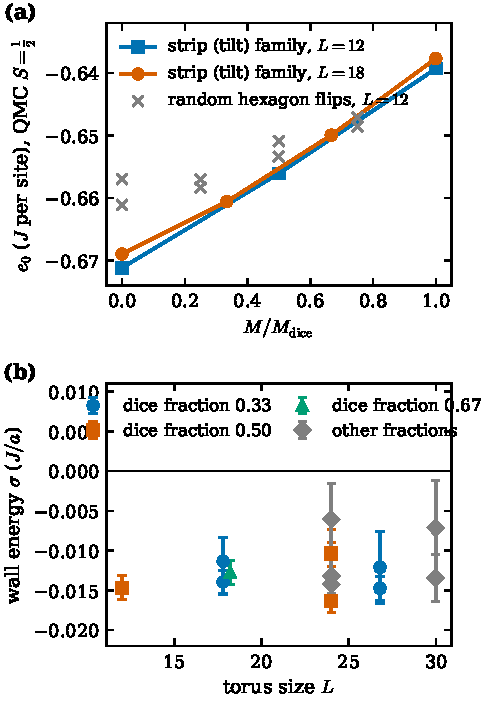
\includegraphics[width=\columnwidth]{figs/fig3_tilt_walls.pdf}
\caption{(a)~QMC ground-state energies ($S=\frac12$) of the tilt family (parallel strips of dice and square tiling) for $L=12$ and $18$, together with tilings obtained by random hexagon flips (crosses). Random flips cost energy at fixed $M$; the classical energy is $-0.5J$ for all points. (b)~Energy per unit length of a dice$|$square wall extracted from the strips, for several dice fractions and torus sizes. All values are negative.}
\label{fig:tilt}
\end{figure}

Figure~\ref{fig:tilt}(a) shows the QMC energy of the tilt family as a function of its moment. The curve is slightly convex: intermediate strip patterns lie \emph{below} the straight line joining the square-type and dice tilings. Subtracting the bulk energies gives the energy per unit length of a dice$|$square wall. It is negative for every width, fraction and system size studied, $\sigma\approx-0.011$ to $-0.015J/a$ [Fig.~\ref{fig:tilt}(b)]. The coordination picture explains the sign. A wall converts rim ($z=3$) and hub ($z=6$) sites of dice into $z=4,5$ sites, which lowers $\sum_i\eps(z_i)$ because $\eps$ is convex. By contrast, random flips at fixed $M$ (crosses) always raise the energy, in agreement with Ref.~\cite{Jagannathan2012}. The sign of $\sigma$ is also opposite to that of the phason-flip walls inside the SDL, whose line energy is $+0.062J/a$~\cite{Jagannathan2013}. Those walls separate two tilings with the same coordination histogram, so they cannot lower $\sum_i\eps(z_i)$; a dice$|$square wall can.

\begin{figure*}[t]
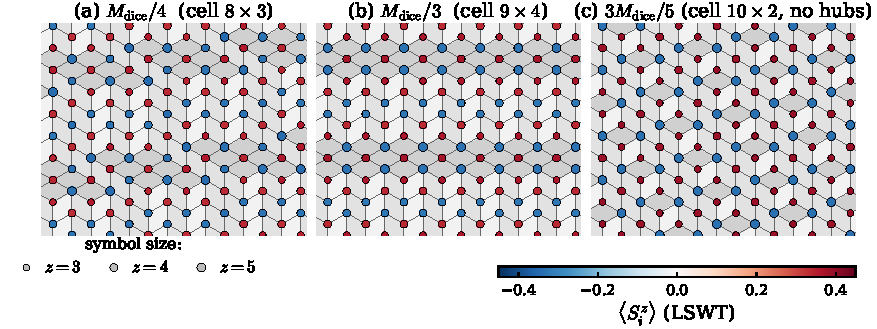
\includegraphics[width=\textwidth]{figs/fig4_crystals.pdf}
\caption{Three periodic tilings of the lower convex hull of $e_0(m)$ (QMC, $S=\frac12$). (a)~$\Md/4$ crystal (cell $8\times3$, shear $s=2$): $z=3$/$z=5$ defects in a square-type background, each with one or two bonded neighbors of opposite curvature. (b)~$\Md/3$ crystal (cell $9\times4$, $s=4$): alternating $z=3$/$z=5$ chains. (c)~$\frac35\Md$ crystal (cell $10\times2$, $s=1$): the hub-free bound of Eq.~(\ref{eq:bound}), $z_3{:}z_4{:}z_5=2{:}1{:}2$, with $z=5$ on every minority site. Rhombi are shaded by orientation. Site color: local moment $\langle S^z_i\rangle$ in the field-polarized ground state (LSWT, thermodynamic limit; red along $h$), which does not change within a plateau; symbol size: coordination $z$.}
\label{fig:crystals}
\end{figure*}

\begin{figure*}[t]
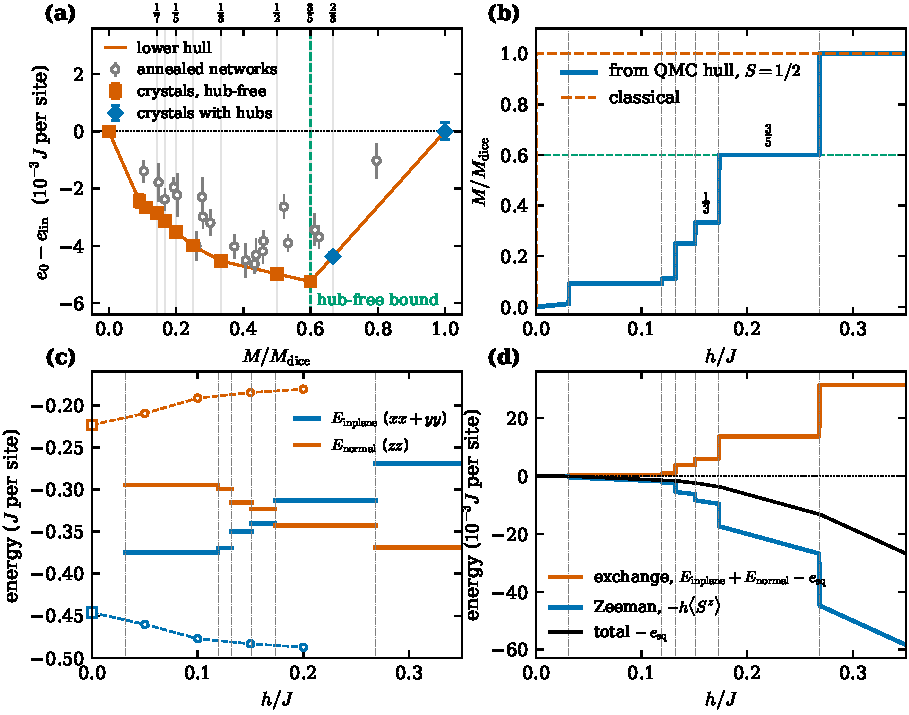
\includegraphics[width=\textwidth]{figs/fig5_staircase.pdf}
\caption{Magnetization staircase ($S=\frac12$, QMC). (a)~Zero-field energy relative to the straight line between the square-type and dice tilings, $e_{\rm lin}(m)=e_{\rm sq}+6m\,(e_{\rm dice}-e_{\rm sq})$. Squares: best hub-free periodic crystal at each $M/\Md$ (Table~\ref{tab:crystals}); diamonds: crystals with hubs. Circles: irregular networks from LSWT annealing at $L=18,24,30$. The line is the lower convex hull, and the dashed vertical line marks the hub-free bound $M=\frac35\Md$, Eq.~(\ref{eq:bound}). (b)~$T=0$ magnetization obtained by minimizing $e_0-hm$ over the hull (solid; the square-type tiling contributes $m=\chi h$), compared with the classical jump (dashed). Dotted vertical lines mark the step fields. (c)~In-plane ($xx+yy$) and normal ($zz$) exchange energy per site along the ground-state path (SSE, $\beta J=36$). Open symbols joined by dashed lines: square-type tiling, with the isotropic values $\frac23e_{\rm sq}$ and $\frac13e_{\rm sq}$ at $h=0$ (squares) and the spin-flop state at $L=24$, also outside its window (circles). (d)~Exchange energy relative to $e_{\rm sq}$, Zeeman energy and their sum along the same path.}
\label{fig:stair}
\end{figure*}

A negative wall energy has a direct consequence. When the field makes dice favorable, the system does not phase-separate into large dice and square domains. It instead gains energy by creating walls. In LSWT on $L=36$ and $48$ tori the energy per straight wall is $\sigma_\infty\approx-0.0088J/a$ for widely separated walls. It becomes about $0.0005J/a$ more negative when the walls are six rows apart, the closest spacing compatible with bipartiteness (Appendix~\ref{app:tests}). Straight walls therefore attract at short distance. The wall picture explains why intermediate structures win, but it does not select the crystal. Superlattices of straight walls lie $2.0$--$2.5\times10^{-3}J$ above the best crystals at the same $m$ (LSWT at $m=1/18$, $1/12$ and $1/9$). The reason is their histogram: the straight-wall superlattice at $\Md/2$ still contains 8\% hubs, whereas the crystal has none. The selection is controlled by the coordination histogram, as in Sec.~\ref{sec:cost}, and the negative wall energy is its consequence rather than an independent cause.

%=====================================================================
\section{Field-driven crystals and the magnetization staircase}\label{sec:field}
%=====================================================================




\begin{table*}[t]
\caption{Periodic crystals on or near the lower hull ($S=\frac12$). $M/\Md=6m$. Coordination counts are per cell, with cells $\mathbf v_1=(p,0)$, $\mathbf v_2=(s,q)$. $\delta e=e_0-e_{\rm lin}$ from QMC, per site, with $N$ the number of sites simulated ($\beta J=36$ on $L=36$ tori or $k\times k$ copies of the cell; dice at $L=\beta J=24$); the square-type reference is the thermodynamic-limit value~\cite{Sandvik1997}. The last columns give the field window in which the crystal is the $T=0$ ground state and the fraction of 4000 hulls, resampled within the QMC errors, in which it appears. Crystals without a window lie on or slightly above a chord of the hull, within about one standard error. The crystals in cells that do not fit an $L=36$ torus were simulated once (one random seed), except $\frac35\Md$.}
\label{tab:crystals}
\begin{ruledtabular}
\begin{tabular}{lcccccc}
$M/\Md$ & cell $(p,q,s)$ & $z_3{:}z_4{:}z_5{:}z_6$ & $\delta e$ ($10^{-3}J$) & $N$ & window ($h/J$) & present\\
\hline
0 & square & $0{:}1{:}0{:}0$ & 0 & $\infty$ & $<0.031$ & 0.97\\
$\frac1{11}$ & $(11,3,4)$ & $2{:}29{:}2{:}0$ & $-2.43(23)$ & 825 & $0.031$--$0.119$ & 0.81\\
$\frac19$ & $(27,1,4)$ & $2{:}23{:}2{:}0$ & $-2.67(16)$ & 972 & $0.119$--$0.132$ & 0.51\\
$\frac17$ & $(14,3,3)$ & $4{:}34{:}4{:}0$ & $-2.85(16)$ & 1050 & --- & 0.12\\
$\frac16$ & $(9,4,4)$ & $4{:}28{:}4{:}0$ & $-3.13(11)$\footnotemark[1] & 1296 & --- & 0.10\\
$\frac15$ & $(10,3,8)$ & $4{:}22{:}4{:}0$ & $-3.51(20)$ & 1080 & --- & 0.40\\
$\frac14$ & $(8,3,2)$ & $4{:}16{:}4{:}0$ & $-3.99(17)$ & 864 & $0.132$--$0.151$ & 0.59\\
$\frac13$ & $(9,4,4)$ & $8{:}20{:}8{:}0$ & $-4.53(9)$\footnotemark[2] & 1296 & $0.151$--$0.173$ & 0.90\\
$\frac12$ & $(6,4,4)$ & $8{:}8{:}8{:}0$ & $-4.98(9)$ & 1296 & --- & 0.48\\
$\frac35$ & $(10,2,1)$ & $8{:}4{:}8{:}0$ & $-5.25(11)$\footnotemark[1] & 1280 & $0.173$--$0.268$ & 1.00\\
$\frac23$ & $(9,4,7)$ & $16{:}6{:}12{:}2$ & $-4.37(12)$ & 1296 & --- & 0.47\\
1 & dice & $2{:}0{:}0{:}1$ & 0 & 576 & $>0.268$ & 1.00\\
\end{tabular}
\end{ruledtabular}
\footnotetext[1]{Mean of three independent runs (random seeds).}
\footnotetext[2]{Mean of two independent runs.}
\end{table*}

\subsection{Exhaustive search of periodic tilings}

Because the energy of a tiling is essentially a function of its coordination histogram, we can scan the complete set of periodic tilings with small unit cells. We took all supercells with up to 48 sites, 403 cell shapes up to the point group $D_6$, enumerated every tiling and retained the bipartite ones, one representative per structural class (Sec.~\ref{sec:methods}). All cell shapes were enumerated completely except 22 cells with 47 and 48 sites, which exceeded our time limit; the 36- and 48-site cells alone contain $2.6\times10^5$--$1.9\times10^7$ tilings each. Ranking by the coordination model is not sufficient for the final selection. It depends only on the histogram, whereas tilings with the same histogram differ by up to $3.5\times10^{-4}J$ (Appendix~\ref{app:tests}). We therefore ranked about $2\times10^4$ candidates with LSWT in the thermodynamic limit (a Bloch calculation on the supercell, which agrees with $L=36$ tori to $10^{-8}J$), and evaluated the hull structures with QMC.

The LSWT hull has points at $M/\Md=\frac1{15},\frac3{41},\frac1{11},\frac19,\frac17,\frac15,\frac14,\frac13,\frac35$ and 1. We evaluated with QMC the crystals from $\frac1{11}$ to $\frac14$, the $\frac35\Md$ crystal, and the crystals at $\Md/6$, $\Md/3$, $\Md/2$ and $2\Md/3$, which have 24- and 36-site cells. The $\frac35\Md$ structure is the tiling that saturates the bound of Eq.~(\ref{eq:bound}): a 20-site cell $(10,2,1)$ with $z_3{:}z_4{:}z_5=8{:}4{:}8$, in which every minority site has $z=5$. Its cell does not fit an $L=36$ torus. A search restricted to cells that do would miss it, together with every crystal whose $M/\Md$ has a denominator with a prime factor other than 2 and 3. In LSWT the $\frac35\Md$ crystal lies $4.29\times10^{-3}J$ below $e_{\rm lin}$, deeper than the $\Md/2$ crystal ($3.89\times10^{-3}J$). The $\Md/2$ crystal falls exactly on the chord between $\frac13$ and $\frac35$ (to $3\times10^{-6}J$), and the $\Md/6$ and $2\Md/3$ structures lie slightly above the LSWT hull.

Figure~\ref{fig:crystals} shows three crystals of the hull, and Fig.~\ref{fig:stair}(a) and Table~\ref{tab:crystals} give the QMC energies of all of them. Crystals whose cells do not fit an $L=36$ torus were simulated on $k\times k$ copies of their cells (Sec.~\ref{sec:methods}). The site colors in Fig.~\ref{fig:crystals} show that the field sorts the moment charges: every site with $z<4$ lies on the majority sublattice $B$ with $\langle S^z_i\rangle\approx0.34$--$0.39$ along $h$, and every site with $z>4$ lies on $A$ with $\langle S^z_i\rangle\approx-0.33$ to $-0.35$, whereas a square-type tiling responds by a spin flop with a uniform $\langle S^z_i\rangle=\chi h$. Three features stand out.

(1)~The deepest point of the hull is the $\frac35\Md$ crystal, $\delta e=-5.25(11)\times10^{-3}J$ (three independent runs). It contains no hubs and saturates the hub-free bound. Its plateau, $0.173J<h<0.268J$, is the widest of the staircase, and it appears in every resampled hull (Table~\ref{tab:crystals}). This is the kink predicted in Sec.~\ref{sec:cost}: up to $\frac35\Md$ the moment is carried by $z=3$ and $z=5$ sites alone, and beyond it hubs are unavoidable.

(2)~The $\Md/2$ and $2\Md/3$ crystals lie on chords of the hull. The $\Md/2$ crystal, $\delta e=-4.98(9)\times10^{-3}J$, coincides with the chord between $\frac13$ and $\frac35$ ($-4.98\times10^{-3}J$ at $m=\frac1{12}$), and the $2\Md/3$ crystal, $-4.37(12)\times10^{-3}J$, with the chord between $\frac35$ and dice ($-4.38\times10^{-3}J$). Each is degenerate, within our resolution, with a coexistence of its neighbors, and each appears in about half of the resampled hulls. The $\Md/2$ crystal has the same coordination histogram as the compensated SDL of Refs.~\cite{Jagannathan2012,Jagannathan2013}. The difference is the arrangement: in the $\Md/2$ crystal the surplus sites are placed on one sublattice, giving $m=1/12$ instead of $0$. The comparison also provides an independent check of Eq.~(\ref{eq:coord}). For the SDL it predicts $E_{\rm LSWT}/N=[\eps(3)+\eps(4)+\eps(5)]/3=-0.6516J$, in agreement with the value $-0.6517(7)J$ obtained by direct LSWT in Ref.~\cite{Jagannathan2013}. The QMC energy of the SDL, $-0.6639J$~\cite{Jagannathan2012}, lies $5.5\times10^{-3}J$ above the square-lattice value, again as Jensen's inequality requires.

(3)~Below $\Md/3$ the hull is dense. The crystals at $M/\Md=\frac1{11},\frac19,\frac17,\frac16,\frac15$ and $\frac14$, all hub-free arrays of $z=3$ and $z=5$ defects in a square-type background, lie within a few $10^{-4}J$ of the chords between their neighbors. Apart from $\frac1{11}\Md$ (81\%), each appears in 10--60\% of the resampled hulls, so the individual low-field plateaus are not resolved by our QMC. The $\Md/3$ crystal, a pattern of alternating $z=3$/$z=5$ chains, is more robust (90\%). In LSWT the hull continues to lower moments, with points down to $\frac1{15}\Md$ and a first step at $0.049J$.

Irregular networks produced by annealing (gray circles) do not go below the hull. They come from 55 LSWT-driven annealing runs at $L=18$ and 106 two-stage (model, then LSWT) runs at $L=24$ and $30$. The runs spanned five tilt sectors, fields $0$--$0.3J$ and two to three random seeds per setting. The best of them, near $M/\Md\approx0.4$--$0.5$, have $\delta e\approx-4.4\times10^{-3}J$, about $0.6\times10^{-3}J$ above the hull; near $M/\Md\approx0.26$--$0.44$ a few lie within one standard error ($3$--$6\times10^{-4}J$) of it. Within our resolution the ground state in a field is therefore a periodic crystal, although nearly degenerate networks exist.

\subsection{Staircase}

At $T=0$ the tiling selected by a field $h$ minimizes $e_0(m)-hm$ (for $S=\frac12$, where the Zeeman energy per site is $-hS_{\rm tot}/N=-hm$), with $-\frac12\chi h^2$ added for the compensated tiling. Minimizing over the hull yields the staircase of Fig.~\ref{fig:stair}(b):
\begin{align*}
0&\xrightarrow{0.031}\tfrac1{11}\xrightarrow{0.119}\tfrac19\xrightarrow{0.132}\tfrac14\\
&\xrightarrow{0.151}\tfrac13\xrightarrow{0.173}\tfrac35\xrightarrow{0.268}1,
\end{align*}
with step fields in units of $J$ and magnetization in units of $\Md$. The classical jump at $h=0^+$ is thus replaced by a staircase with two distinct parts. Between $h\approx0.03$--$0.05J$ and $0.15J$ the magnetization rises to $\Md/4$ in several steps, each a denser packing of defects. The order of these steps is not fixed by our data (feature 3), and the onset field is the least certain number: the QMC error of $2.3\times10^{-4}J$ at $\frac1{11}\Md$ moves it by $0.015J$. Above it come the $\Md/3$ plateau ($0.022J$ wide) and the $\frac35\Md$ plateau ($0.095J$ wide), before the jump to dice. This staircase is established within the searched space: periodic cells with up to 48 sites, plus the annealed networks. It is not a proof over all tilings. Each step corresponds to a first-order change of the \emph{lattice} and not only of the spin state.

Figures~\ref{fig:stair}(c) and \ref{fig:stair}(d) decompose the energy along this path. We measure the two parts of the exchange energy directly in SSE: $E_{\rm inplane}=-\langle n_{\rm od}\rangle/(\beta N)$ from the number of off-diagonal operators, and $E_{\rm normal}$ from the diagonal energy, which agrees with the equal-time estimator. Within a plateau both are independent of $h$. The exchange energy rises in steps, by $0.032J$ in total, and the Zeeman energy $-hm$ pays for each step. The first step also reorients the order. In the square-type tiling the staggered moment lies perpendicular to $h$ (spin flop), so $E_{\rm normal}\approx-0.18$ to $-0.21J$ is a transverse correlation. In the ferrimagnetic crystals the moment is collinear with $h$, and $E_{\rm normal}$ is the longitudinal one, $-0.30J$ for $\frac1{11}\Md$. Along the staircase $E_{\rm normal}$ grows to $-0.37J$ and $E_{\rm inplane}$ shrinks from $-0.37$ to $-0.27J$, as the moments become more nearly classical. At $h=0$ the square-type ground state is a spin singlet with isotropic correlations, so that $E_{\rm normal}=e_{\rm sq}/3$.

\emph{Robustness.} We assess the staircase in three ways. (i)~\emph{Statistical errors.} Resampling all QMC energies within their errors (4000 samples, last column of Table~\ref{tab:crystals}) keeps the $\frac35\Md$ plateau and the jump to dice in every sample, with step fields $0.176\pm0.006J$ and $0.269\pm0.005J$. The $\Md/3$ plateau appears in 90\% of the samples, with lower edge $0.152\pm0.009J$. The low-field crystals appear in 10--81\%, and the $\Md/2$ and $2\Md/3$ crystals, which lie on chords, in about half of the samples. The existence of the individual low-field plateaus is therefore not established, but the field range they occupy is. In 3\% of the samples the $\frac1{11}\Md$ crystal lies below the square-type tiling at $h=0$; its zero-field energy is above that of the square-type tiling by $0.44(23)\times10^{-3}J$, i.e., by two standard errors. (ii)~\emph{System size.} The $\Md/2$ deviation is $-5.3(4)$ and $-4.98(9)\times10^{-3}J$ at $L=24$ and $36$, and $-4.8\times10^{-3}J$ at $L=12$ relative to $L=12$ references (Table~\ref{tab:spinS}). The dice reference agrees between $L=18$ and $24$ to $10^{-4}J$, and the square-type reference is taken in the thermodynamic limit (Sec.~\ref{sec:methods}). In LSWT the crystal energies at $L=36$, and on the $k\times k$ clusters, coincide with the thermodynamic limit. (iii)~\emph{Cell size.} The $\frac35\Md$ crystal has a 20-site cell and is the lowest tiling at the bound that we find in cells of up to 48 sites. The bound itself, Eq.~(\ref{eq:bound}), holds for all tilings, and the leading-order optimum at the bound is the histogram $2{:}1{:}2$. Larger cells could therefore lower the $\frac35\Md$ point only through arrangement energies, of order $10^{-4}J$, and not at leading order. They may still add hull points elsewhere, most likely at low moment, where the hull is dense.

The Lieb--Mattis theorem fixes $S_{\rm tot}=M$ at $h=0$. Because $S^z_{\rm tot}$ is conserved on a fixed graph and states with larger $S^z_{\rm tot}$ are separated by a magnon gap, the spin ground state stays pinned at $S^z_{\rm tot}=M$ throughout each plateau.

\subsection{A lattice gas of curvature defects}\label{sec:gas}

\begin{figure}[t]
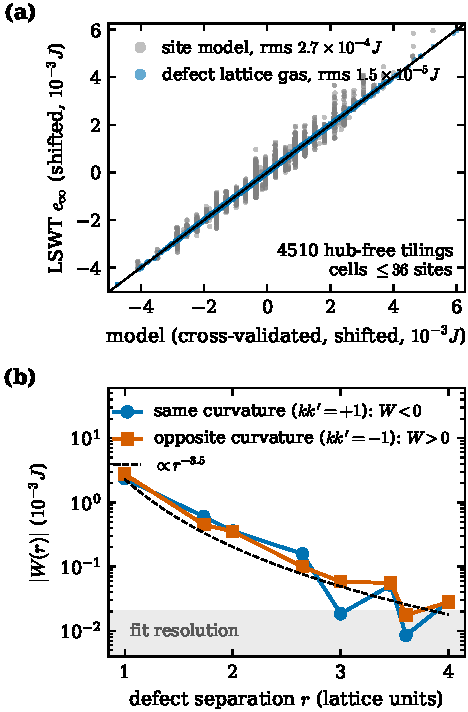
\includegraphics[width=\columnwidth]{figs/fig11_defectgas.pdf}
\caption{Defect lattice gas, Eq.~(\ref{eq:gas}), fitted to thermodynamic-limit LSWT energies ($S=\frac12$) of all structurally distinct hub-free periodic tilings with cells of up to 36 sites. (a)~Cross-validated prediction vs LSWT: site model, Eq.~(\ref{eq:coord}), refitted to the same set (gray), and the lattice gas with pair terms up to $r=\sqrt7$ (blue). (b)~Magnitude of the pair energy $W$ for defects of the same (circles) and opposite (squares) curvature, averaged over the two sublattice relations; bonded nearest neighbors are included at $r=1$. Same-curvature pairs attract and opposite-curvature pairs repel. The dashed line is $\propto r^{-3.5}$; the shaded band marks the resolution of the fit.}
\label{fig:gas}
\end{figure}

The site model treats every $z\ne4$ site independently and misses the arrangement energies that decide the low-field plateaus; on hub-free tilings its residual is $2.7\times10^{-4}J$. We therefore describe a hub-free tiling as a lattice gas of curvature defects, the sites with $k_i=4-z_i=\pm1$, each on a sublattice $\eta_i=\pm1$, and fit
\begin{equation}
\frac{E_{\rm LSWT}}{N}=e_{\rm sq}+\eps_d\,\rho_d+c'_m\,m+\frac1N\sum_{i<j}W(r_{ij};k_ik_j,\eta_i\eta_j),
\label{eq:gas}
\end{equation}
where $\rho_d$ is the defect density. The pair energy $W$ depends on the distance and on whether the two defects have the same curvature and lie on the same sublattice, and bonded and unbonded nearest neighbors are distinguished. We fit Eq.~(\ref{eq:gas}) to the Bloch-LSWT energies of all 4510 structurally distinct hub-free tilings with cells of up to 36 sites, keeping pairs up to $r=\sqrt7$ [extending the cutoff to $r=4$, Fig.~\ref{fig:gas}(b), does not lower the residual]. The cross-validated residual is $1.5\times10^{-5}J$, 18 times smaller than for the site model [Fig.~\ref{fig:gas}(a)]. On 74 hub-free 48-site structures that were not used in the fit it is $2.1\times10^{-5}J$. The fitted parameters are $\eps_d=6.92(2)\times10^{-3}J$ and $c'_m=1.99(3)\times10^{-3}J$, and three rules follow from the pair energies.

\emph{(1) Sign.} In 14 of the 16 pair channels ${\rm sign}\,W=-k_ik_j$, i.e., defects of the same curvature attract and defects of opposite curvature repel; the two exceptions are within the resolution. Bonded nearest neighbors dominate, with $W=-3.24(2)\times10^{-3}J$ for like and $+4.39(2)\times10^{-3}J$ for unlike pairs. The unlike value, which we denote $W_1^{\rm unlike}$, is close to the Ising-expansion contact energy, $+4.8\times10^{-3}J$, and the like value lies between the Ising values for $(3,3)$ and $(5,5)$ contacts, $-8.3$ and $-3.0\times10^{-3}J$ (Sec.~\ref{sec:ising}). The field, which couples to the staggered curvature [Eq.~(\ref{eq:stagK})], is what sorts the curvature onto the two sublattices (Appendix~\ref{app:geom}); the pair energies then decide how the sorted defects are arranged.

\emph{(2) Range.} $|W|$ decreases by a factor of about 30 between $r=1$ and $r=3$ [Fig.~\ref{fig:gas}(b)]. Beyond $r\approx3$ the couplings are below $2\times10^{-5}J$. The four resolved shells are compatible with a power law $\propto r^{-3.5}$, but two of them lie close to the resolution of the fit, so we do not attach significance to the exponent. Resolving $W$ into a curvature channel ($\propto k_ik_j$) and a moment channel ($\propto q_iq_j$, with $q_i=-\eta_ik_i$ the moment charge of Eq.~(\ref{eq:charge})) shows that the curvature channel dominates at short range, while at $r=2$ and $\sqrt7$ the moment channel is comparable and repulsive between equal moments ($+0.10$ and $+0.08\times10^{-3}J$). This is the sign expected for the magnon-mediated interaction between uncompensated moments, which is expected to decay as $r^{-3}$ for phason flips in the staggered dice lattice~\cite{Jagannathan2012}. In a polarized crystal all moments are equal, so this tail is repulsive and further favors evenly spaced dipoles.

\emph{(3) Packing.} Along the hull the defects pack more closely at each step. The number of bonded contacts with defects of opposite curvature rises from 0 per defect ($\frac1{11}\Md$, $\frac19\Md$), 0.5 ($\frac17\Md$) and 1.0 ($\Md/6$, $\Md/5$) through 1.5 ($\Md/4$) and 2.0 (alternating chains, $\Md/3$) to 2.75 ($\Md/2$) and 3.0 ($\frac35\Md$). The number of unbonded nearest-neighbor contacts between like-curvature defects rises from 0 to 1.5. At the lowest densities the defects have no neighbor of opposite curvature (all of them at $\frac1{11}\Md$ and $\frac19\Md$, half at $\frac17\Md$, a quarter at $\Md/6$): dilute defects stay apart, as the repulsion between bonded unlike defects requires. At higher density unlike contacts become unavoidable, and the crystals combine them with attractive like contacts. In the $\frac35\Md$ crystal each $z=3$ site has three $z=5$ neighbors, and each $z=5$ site three $z=3$ and two $z=4$ neighbors. Each step field is set by the cost of the next contact divided by the moment it adds. Within each $m$, the model ranks the polarized structures in the same order as LSWT (Spearman correlation 0.93--0.98) and picks the same lowest structure.

The model also gives the onset of the staircase. Two field-aligned defects that do not touch cost $2\eps_d+c'_m/4=14.3\times10^{-3}J$ and carry $mN=\frac14$, so the first step is expected near $h\approx0.057J$; a bonded pair would cost $W_1^{\rm unlike}$ more and give $0.075J$. These estimates neglect the energy $\frac12\chi h^2$ that the square-type tiling gains by its spin flop. For a crystal of moment $m$ this shifts the step up by $\chi h^2/(2m)$, about $0.002J$ for $\frac1{11}\Md$ at $h\approx0.03J$. The LSWT hull indeed begins with dilute crystals of separated defects, with a first step at $0.049J$. In QMC the most dilute crystal we evaluated, $\frac1{11}\Md$, gives $0.031\pm0.015J$.

\emph{Dilute limit and the limits of finite cells.} A cell of $N_c$ sites cannot host a crystal with $0<m<1/(2N_c)$, so crystals more dilute than those enumerated, such as $\frac1{13}\Md$ or $\frac1{17}\Md$, are missing from our hull. Their energies relative to their neighbors would also be below the finite-cluster accuracy of LSWT ($4\times10^{-5}J$) and far below the QMC errors. The onset field, however, does not depend on them. Because $e_0(m)$ is convex, the first step leads from the square-type tiling to the crystal with the smallest $[e_0(m)-e_{\rm sq}]/m$, and this ratio decreases toward the dilute limit
\begin{equation}
h_c=\lim_{m\to0}\frac{e_0(m)-e_{\rm sq}}{m},
\label{eq:hc}
\end{equation}
which is the cost of one isolated, field-aligned $z=3$/$z=5$ pair divided by its moment and does not depend on which dilute crystals exist. Between $h_c$ and the field at which the most dilute evaluated crystal appears, the magnetization rises through all the missing crystals. The width of this range is set by the interaction between distant defects. A repulsive tail, such as the $r^{-3}$ magnon-mediated interaction between equal moments, makes every density appear and gives $m\propto(h-h_c)^{2/3}$, while an attractive tail makes the rise a single jump. In LSWT the ratio $[e_0(m)-e_{\rm sq}]/m$ is $0.0492$, $0.0495$, $0.0508$ and $0.0542J$ at $M/\Md=\frac1{15},\frac3{41},\frac1{11}$ and $\frac19$: it saturates below $\frac1{11}\Md$, so separated defects interact only weakly, consistent with $|W|<2\times10^{-5}J$ beyond $r\approx3$. In LSWT the missing dilute crystals are therefore confined to a field range of order $10^{-3}J$ above $h_c\approx0.049J$, and the magnetization reaches $\frac1{11}\Md$ within $0.007J$ of $h_c$. Whether this rise is continuous or a jump cannot be decided at our resolution, and it does not affect the staircase at the scale of Fig.~\ref{fig:stair}. Applying the same saturation, scaled by the LSWT-to-QMC factor of about $1.3$, to the QMC values at $\frac1{11}\Md$ and $\frac19\Md$ gives $h_c=0.036\pm0.007J$, consistent with the step into $\frac1{11}\Md$. This is below the LSWT onset, whereas QMC step fields at higher moment exceed the LSWT ones by factors of 1.2--1.4 (Appendix~\ref{app:lswt}). Given the uncertainty of the compensated reference (Sec.~\ref{sec:methods}), which enters $h_c$ directly, we do not regard this difference as significant. Finally, because $W$ is short ranged, neighboring packing stages differ by contact numbers only, and their energies differ by a few $10^{-4}J$ from the chords between them. This is why the low-field part of the hull is dense and shallow, and why our QMC, with errors of $1$--$2\times10^{-4}J$, resolves the field range of these steps but not each step individually.



%=====================================================================
\section{Fluctuations, entanglement and spectroscopic signatures}\label{sec:fluct}
%=====================================================================

\begin{figure}[t]
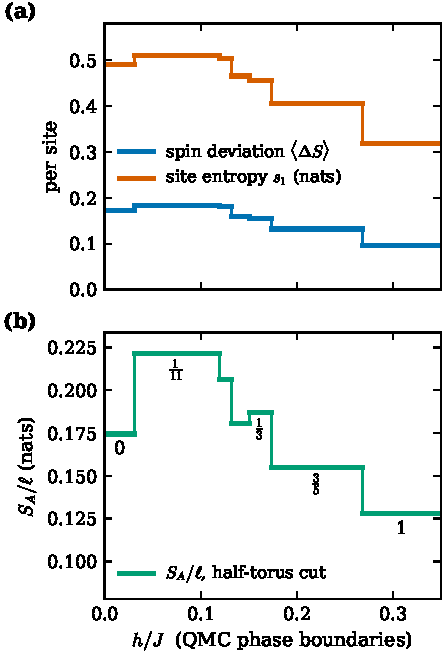
\includegraphics[width=\columnwidth]{figs/fig6_fluct.pdf}
\caption{Quantum-fluctuation measures of the LSWT ground state ($S=\frac12$) of the crystal selected at each field, using the QMC phase boundaries ($L=36$ tori, or $L=24$--$60$ tori for cells that do not fit $L=36$). (a)~Mean spin deviation $\langle\Delta S\rangle=\langle a^\dagger a\rangle$ and single-site entanglement entropy. (b)~Gaussian entanglement entropy of half the torus per unit boundary length, from the covariance matrices of the quadratures. Plateau labels give $M/\Md$.}
\label{fig:fluct}
\end{figure}

\begin{figure*}[t]
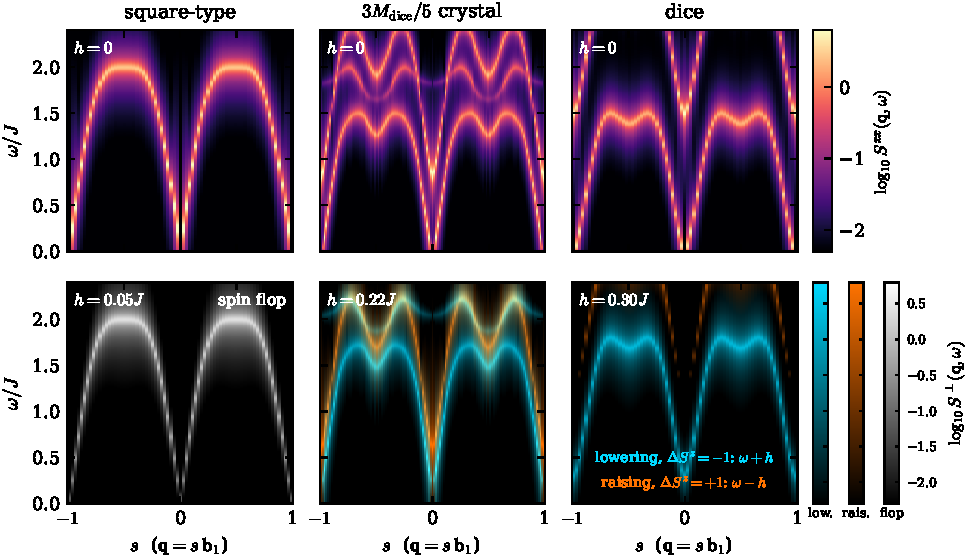
\includegraphics[width=\textwidth]{figs/fig7_sqw.pdf}
\caption{LSWT transverse dynamical structure factor ($S=\frac12$, Lorentzian broadening $0.03J$, logarithmic scale) along $\mathbf q=s\,\mathbf b_1$, where $\mathbf b_1$ is a reciprocal vector of the triangular lattice ($L=36$; $L=60$ for the $\frac35\Md$ crystal). Top row: $S^{xx}(\mathbf q,\omega)$ at $h=0$ for the square-type tiling (a single sharp magnon branch), the $\frac35\Md$ crystal (backfolded minibands and gaps set by its 20-site cell) and dice (a Goldstone branch plus the dispersionless band near $1.5J$ that comes from the rim sites). Bottom row: response transverse to a field inside each plateau. For the ferrimagnetic crystals the channels $\Delta S^z=-1$ (cyan, shifted to $\omega+h$) and $\Delta S^z=+1$ (orange, $\omega-h$) are shown separately. The square-type tiling is in the spin-flop state and shows a single unsplit branch (white). In the bottom row the hue identifies the channel and the brightness gives the intensity on the same logarithmic scale as in the top row (keys at right).}
\label{fig:sqw}
\end{figure*}

Because the spin state within a plateau does not change with $h$, the quantum-fluctuation content of the ground state changes only at the steps, where the lattice changes. Figure~\ref{fig:fluct} follows three measures along the staircase. The mean spin deviation rises slightly at the first steps, to $0.18$, and then decreases, to $0.155$ ($\Md/3$), $0.132$ ($\frac35\Md$) and $0.095$ (dice), and the single-site entanglement entropy falls from $0.49$ to $0.32$. The field thus reduces quantum fluctuations in discrete steps, by selecting lattices with more $z=3$ sites on the majority sublattice, whose moments are the most nearly classical (their mean spin deviation falls from $0.20$ in the $\frac19\Md$ crystal to $0.11$ in the $\frac35\Md$ crystal and $0.07$ in dice). The half-system entanglement per unit boundary length is not monotonic. It rises by up to 27\% at the first steps, where isolated defects add soft local modes, returns to the square-type value near $\Md/3$, and then falls, by 11\% at $\frac35\Md$ and by 26\% at dice relative to the square-type tiling. The values refer to finite tori with zero modes excluded, and differences of a few percent between crystals simulated at different $L$ are not significant. This is the mirror image of the zero-field selection.

The crystals can be distinguished spectroscopically [Fig.~\ref{fig:sqw}]. The square-type tiling shows a single linearly dispersing magnon branch. The dice tiling combines a Goldstone branch with the dispersionless band near $\omega\approx1.5J$ localized on the rims~\cite{Sutherland1986}. The $\frac35\Md$ crystal shows backfolded minibands with small gaps at the zone boundaries of its 20-site cell. Its low-energy branch is square-like, and its upper spectral weight is spread over a band of nearly flat modes. These features give a direct fingerprint of each plateau in inelastic neutron scattering or in magnon spectroscopy of engineered structures.

A field separates the two kinds of tiling (Fig.~\ref{fig:sqw}, bottom row). In a ferrimagnetic crystal the moment is locked along $h$, the Zeeman term commutes with $H_{\mathcal T}$, and every magnon carries $\Delta S^z=\pm1$. The spectrum is therefore split rigidly, $\omega\to\omega\mp h$, and the two sets of branches appear in different polarization channels. The Goldstone mode acquires the gap $h$. The moment-raising branch has the LSWT gap $\Delta_+=0.12$, $0.15$, $0.32$, $0.43$, $0.66$, $0.82$, $0.90$ and $1.50J$ for the $\frac1{11}\Md$, $\frac19\Md$, $\Md/4$, $\Md/3$, $\Md/2$, $\frac35\Md$, $2\Md/3$ and dice crystals, roughly $8Jm$. A plateau is stable against magnon condensation as long as $h<\Delta_+$, i.e., $\Delta_+$ must exceed the upper edge of its window. This holds by a wide margin for every crystal on the path except $\frac1{11}\Md$, whose LSWT gap ($0.120J$) coincides with the upper edge of its QMC window ($0.119J$); for this crystal the nature of the upper edge, a change of lattice or a magnon condensation, is not determined. Within its window each crystal therefore has zero differential susceptibility, and each step is a change of lattice, not a magnon condensation. The square-type tiling responds instead by a spin flop. Its magnons are not eigenstates of $S^z$, and the uniform mode acquires the gap $h$, so that $\chi\simeq0.065J^{-1}$ remains finite. In a field the two kinds of tiling therefore differ in symmetry. The spin-flop state breaks the $U(1)$ symmetry about $h$ and keeps one linearly dispersing Goldstone mode. A ferrimagnetic crystal is collinear with $h$, preserves this symmetry, and has no gapless mode: its former Goldstone mode is gapped by $h$. In the limit $h\to0$ the difference becomes one of Goldstone-mode type. In the compensated tiling the two broken generators have a vanishing commutator, $\langle[S^x_{\rm tot},S^y_{\rm tot}]\rangle=i\langle S^z_{\rm tot}\rangle=0$, and give two linearly dispersing (type-A) modes. In a ferrimagnetic crystal the commutator is $iM\neq0$, the two generators form a canonical pair, and a single quadratically dispersing (type-B) mode remains~\cite{WatanabeBrauner2011,Watanabe2012,Hidaka2013}.

%=====================================================================
\section{Dependence on spin length}\label{sec:spinS}
%=====================================================================

\begin{figure}[t]
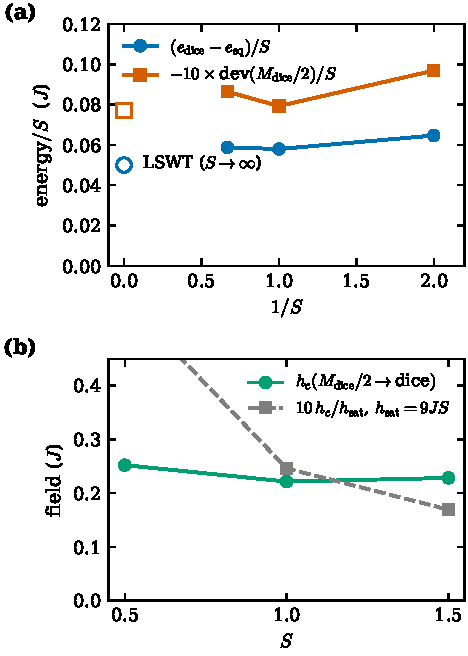
\includegraphics[width=\columnwidth]{figs/fig8_spinS.pdf}
\caption{Spin-$S$ QMC ($L=12$, $\beta JS=12$). (a)~Selection energies per unit $S$: dice minus square-type (circles) and the $\Md/2$ deviation (squares, $\times(-10)$). Open symbols: LSWT ($S\to\infty$). Both approach finite limits, i.e., selection energies scale as $JS$. (b)~The field at which the $\Md/2$ crystal gives way to dice at this system size (circles) is $S$-independent in units of $J$. Relative to the saturation scale, the intermediate region therefore shrinks as $1/S$ (squares).}
\label{fig:spinS}
\end{figure}

\begin{table}[b]
\caption{Spin-$S$ dependence (QMC, $L=12$). Energies per site in units of $J$.}
\label{tab:spinS}
\begin{ruledtabular}
\begin{tabular}{lccc}
$S$ & $(e_{\rm dice}-e_{\rm sq})/S$ & $\delta e(\Md/2)/S$ & $h_c(\Md/2\to{\rm dice})$\\
\hline
$\frac12$ & 0.065 & $-0.0097$ & 0.25\\
1 & 0.058 & $-0.0079$ & 0.22\\
$\frac32$ & 0.059 & $-0.0086$ & 0.23\\
LSWT & 0.050 & $-0.0077$ & ---\\
\end{tabular}
\end{ruledtabular}
\end{table}

Classically the selection energy vanishes, and in spin-wave theory it is of order $JS$, whereas the exchange energy is of order $JS^2$. QMC for $S=\frac12$, $1$ and $\frac32$ confirms this scaling (Fig.~\ref{fig:spinS} and Table~\ref{tab:spinS}). The ratios $(e_{\rm dice}-e_{\rm sq})/S$ and $\delta e(\Md/2)/S$ are nearly constant and of the same size as the LSWT values ($S\to\infty$). (The $\frac35\Md$ crystal does not fit an $L=12$ torus, so we use the $\Md/2$ crystal, which lies on the hull chord next to it, as the representative hub-free crystal.) The same $JS$ scaling follows from Eq.~(\ref{eq:ising}), whose bond terms depend on $S$ only through the shift $1/S$ in the denominator. Both the energy differences and the Zeeman energy $hM\propto hS$ are linear in $S$, so the step fields are expected to be $S$-independent in units of $J$. We have checked this for one step: the field at which the $\Md/2$ crystal gives way to dice is $0.22$--$0.25J$ for all three spins. Measured against the saturation field, which grows as $JS$ ($8JS$ for the square lattice and $9JS$ for dice in LSWT), the intermediate region therefore shrinks as $1/S$. The staircase is a genuinely quantum phenomenon, most pronounced for $S=\frac12$; within our $L=12$ data, the $\Md/2\to$dice field varies by about 12\% between $S=\frac12$ and $\frac32$.

%=====================================================================
\section{Discussion}\label{sec:disc}
%=====================================================================

\emph{Height-model interpretation.} Appendix~\ref{app:geom} makes the height representation concrete: Eq.~(\ref{eq:coord}) is an effective height model whose potential is a convex function of the local Gaussian curvature of the lifted surface. The field acts as a chemical potential for the sublattice imbalance. In this language the plateaus are \emph{locked} phases of the height model, commensurate crystals analogous to the ordered phases of quantum dimer models~\cite{Rokhsar1988,Moessner2001}, in particular of the hexagonal-lattice dimer model, whose dimer coverings are the lozenge tilings~\cite{MoessnerSondhiChandra2001}. The staircase is analogous to the devil's staircases of competing-interaction systems~\cite{Bak1982}, but here the underlying potential is set by the convexity of $\eps(z)$ and not by an imposed long-range interaction. Our data establish a robust skeleton, the $\frac35\Md$ plateau, the $\Md/3$ plateau and the jump to dice, together with a dense set of narrow steps at low field. In the low-field part the energies of successive packing stages differ from the chords between them by a few $10^{-4}J$. Near the onset, the dilute crystals that finite cells cannot host are confined to a field range of order $10^{-3}J$ above $h_c$ (Sec.~\ref{sec:gas}); whether they form a complete devil's staircase there, as a repulsive long-range tail would imply, is open but immaterial at the scale of the observable staircase.

\emph{Relation to known plateaus.} Magnetization plateaus in quantum magnets usually arise from a crystal of magnetic excitations on a \emph{fixed} lattice~\cite{Kageyama1999,Honecker2004}. Plateaus can also be stabilized by a coupling to the lattice, as in the half-magnetization plateau of the pyrochlore antiferromagnet, where a structural distortion modulates the exchange constants~\cite{PencShannonShiba2004}. In that mechanism the bond network keeps its topology and only the bond strengths change. Here the plateau is a crystal of the lattice itself: the topology of the network changes from step to step, all bonds keep the same $J$, and the spin state on each plateau is the Lieb--Mattis ground state of that network. The mechanisms could coexist if bond strengths are also varied. Studying that would require going beyond the uniform-$J$ model~(\ref{eq:H}).

\emph{Platforms.} Three classes of system make the graph of exchange bonds a design or growth variable. (i)~\emph{$\pi$-magnetic nanographenes}, whose ground-state spin is set by the bipartite network of $\pi$ orbitals through sublattice imbalance and topological frustration, and whose building blocks can be fused into extended chains and networks~\cite{Mishra2020,Mishra2021}. (ii)~\emph{Atom-by-atom spin arrays} on surfaces, which realize arbitrary two-dimensional coupling graphs and allow local spectroscopy of spin excitations~\cite{Khajetoorians2019}. (iii)~\emph{Programmable quantum simulators}, such as Rydberg arrays, in which the connectivity is reconfigurable and antiferromagnetic correlations on hundreds of sites have been measured~\cite{Scholl2021}. These experiments realize Ising-type antiferromagnets, so a Heisenberg version of Eq.~(\ref{eq:H}) would require a different encoding. In (ii), and in (iii) once Heisenberg couplings are encoded, the energies $e_0(m)$ of different tilings can be compared directly, and the $\frac35\Md$ crystal, with a 20-site cell, is a concrete target structure. In (i) the step fields, $0.03$--$0.27J$, and the melting temperature of the $\Md/2$ crystal in the effective model, $0.02$--$0.03J$, give the relevant scales once $J$ is known. In small systems ($N\sim10^2$) a further scale enters: a few uncompensated defects in a compensated background carry a size-dependent energy $\approx\alpha|\mu|/N$, with $\alpha\approx3.4J$ for the staggered dice lattice in our LSWT, ED and QMC checks, related to the low-energy states of locally uncompensated regions in diluted antiferromagnets~\cite{WangSandvik2006}. This is comparable to the step fields at $N\sim10^2$ and would shift the lowest steps in finite arrays.

\emph{Limitations.} (a)~The enumeration is exhaustive for cells of up to 48 sites (LSWT screening), except for 22 cells with 47 and 48 sites. The hull structures were evaluated with QMC on clusters of 825--1296 sites. Larger cells may add steps or shift boundaries, most likely at low field. In particular, crystals more dilute than $\frac1{15}\Md$ cannot be hosted by our cells; the dilute-limit argument of Sec.~\ref{sec:gas} confines them to about $10^{-3}J$ above the onset field $h_c$, which itself is a property of isolated defect pairs and not of the cells. The hub-free bound and its saturation by the $\frac35\Md$ crystal do not depend on cell size. (b)~Below $\Md/3$, and for the $\Md/2$ and $2\Md/3$ crystals, the margins are a few $10^{-4}J$, comparable to the QMC errors, and the new low-field crystals were simulated with a single random seed. That the deepest crystal has a cell incompatible with an $L=36$ torus shows that conclusions at the sub-$10^{-3}J$ level depend on the completeness of the search. (c)~The coordination model is used only for screening. The defect lattice gas reaches $1.5\times10^{-5}J$, but it is fitted to LSWT, which underestimates the QMC deviations by a density-dependent factor of 1.2--1.5, and it covers only hub-free tilings. (d)~The finite-temperature results refer to an effective tiling model at fixed tilt without thermal spin fluctuations. The quoted $T_m$ is a scale of that model, and the non-recrystallization is kinetic trapping. (e)~Irregular networks were generated with a model-assisted annealing that is not exhaustive. No irregular network we evaluated with QMC lies below the periodic hull, but a few lie within one standard error of it. (f)~The QMC energies were not extrapolated in $\beta$ (Sec.~\ref{sec:methods}). (g)~The model contains only uniform nearest-neighbor exchange. Further-neighbor couplings, or a dependence of $J$ on the local environment, of order $10^{-4}J$ would reorder the low-field crystals, whose margins are of that size. The $\frac35\Md$ plateau, about $0.1J$ wide and resting on the leading-order convexity of order $10^{-2}J$, should survive perturbations that are small compared with these scales.

%=====================================================================


\section{Conclusion}\label{sec:concl}
%=====================================================================

We have shown that the classically degenerate family of lozenge-tiling networks is organized, quantum mechanically, by one simple rule: the zero-point energy is a convex function of the site coordination. An expansion about the Ising limit shows where the rule comes from: a site with more bonds has more channels for quantum fluctuations, but each fluctuation frustrates more bonds, so the gain saturates. This rule selects the uniform square-type tiling at zero field, gives dice$|$square-type walls negative energy, and, in competition with the Zeeman energy of the Lieb moment, stabilizes, within the searched space, a staircase of periodic crystals rather than the classical jump or a disordered network. Because a moment is carried most cheaply by $z=3$ and $z=5$ sites, hubs are avoided as long as possible, and bond counting together with Lieb's theorem limits hub-free tilings to $M\le\frac35\Md$. A crystal with a 20-site cell, in which every minority site is fivefold, saturates this bound. It is the deepest point of the energy hull and the central object of this work, stable over $0.173J<h<0.268J$ for $S=\frac12$, and its field window is set by selection energies that scale as $JS$. Below it the staircase is dense: crystals of $z=3$ and $z=5$ defects follow one another in narrow windows, held in place by a short-ranged attraction between curvature defects of the same sign and a repulsion between defects of opposite sign. Geometrically, zero field selects folded, curvature-free surfaces, and the field crumples them with sorted conical defects, because the Lieb moment is exactly the sublattice-staggered Gaussian curvature; the $\frac35\Md$ crystal is the densest packing of sublattice-sorted $\pm\pi/2$ cones and saddles. These results identify quantum order by disorder acting on the geometry of the exchange network itself. They also provide concrete target structures and energy scales for nanographene networks, atom-by-atom spin arrays and quantum simulators, in which that geometry can be designed.

\section*{Data availability}
The data that support the findings of this article are openly available~\cite{DataRepo}. The repository contains the SSE QMC, LSWT and enumeration codes, the crystal tilings, the QMC logs and the figure scripts.

\begin{acknowledgments}
This research was supported by the National Research Foundation (NRF) of Korea funded by the Korean Government (NRF-2023R1A2C1006050). The authors used Claude (Anthropic) to assist with writing code for the numerical computations and figures and with editing the manuscript; all results were checked by the authors, who take full responsibility for the content.
\end{acknowledgments}



\appendix

%=====================================================================
\section{Geometric interpretation: folded and crumpled surfaces}\label{app:geom}
%=====================================================================

\begin{figure*}[t]
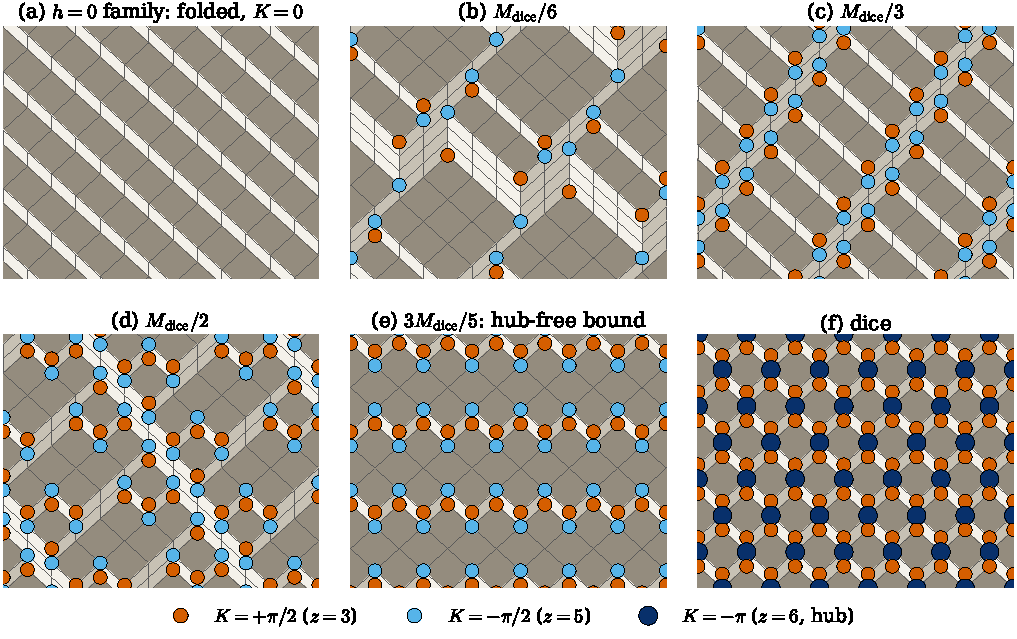
\includegraphics[width=\textwidth]{figs/fig10_curvature.pdf}
\caption{Tilings lifted to stepped surfaces in $\mathbb Z^3$ (orthographic view, tilted by $12^\circ$ from $[111]$; faces shaded by orientation). Colored dots mark vertices with nonzero discrete Gaussian curvature $K_i=2\pi-\frac\pi2 z_i$. (a)~A zero-curvature tiling from the degenerate $h=0$ family: two facets joined by straight folds, $K_i=0$ everywhere. (b)--(e)~Crystals of the hull at $M/\Md=\frac16,\frac13,\frac12,\frac35$. Positive curvature ($z=3$) sits only on the majority sublattice and negative curvature ($z=5$) only on the minority sublattice. The $\frac35\Md$ crystal (e) is the densest packing of sorted $\pm\pi/2$ vertices, Eq.~(\ref{eq:bound}); its surface is tilted by $30^\circ$. (f)~Dice: $+\pi/2$ cones and $-\pi$ hubs.}
\label{fig:curv}
\end{figure*}

\emph{Definitions.} Every lozenge tiling is the projection along $[111]$ of a stepped surface $\Sigma$ made of unit squares of the cubic lattice~\cite{Kenyon2006}. We lift the tiling by assigning the steps $+\mathbf e_x$, $+\mathbf e_y$, $+\mathbf e_z$ to the bond directions $\mathbf a_1$, $\mathbf a_2-\mathbf a_1$, $-\mathbf a_2$ (whose sum vanishes). Each lozenge becomes a unit square face, and the tiling graph becomes the edge skeleton of $\Sigma$. We verified that the lift is single-valued for all structures shown. Around a vertex of coordination $z_i$ there are exactly $z_i$ faces, each contributing a right angle, so the discrete Gaussian curvature (angle deficit) is
\begin{equation}
K_i=2\pi-\frac{\pi}{2}\,z_i=\tfrac{\pi}{2}\,(4-z_i).
\label{eq:K}
\end{equation}
Sites with $z=3,4,5,6$ are cones ($+\pi/2$), flat points ($0$), saddles ($-\pi/2$) and strong saddles ($-\pi$). Two exact identities follow. First, $\langle z\rangle=4$ is the discrete Gauss--Bonnet theorem on the torus, $\sum_iK_i=0$. Second, inserting Eq.~(\ref{eq:K}) into Eq.~(\ref{eq:charge}) gives
\begin{equation}
N_B-N_A=-\frac{1}{2\pi}\sum_i\eta_iK_i,\qquad S_{\rm tot}=\frac{S}{2\pi}\Big|\sum_i\eta_iK_i\Big| ,
\label{eq:stagK}
\end{equation}
with $\eta_i=+1$ ($-1$) on sublattice $A$ ($B$). The total curvature always vanishes, and the Lieb moment is its sublattice-staggered part. The same sum is the coefficient of the uncompensated Berry phase, $iS\sum_i\eta_i\,\omega[\mathbf n]$ for $\mathbf n_i=\eta_i\mathbf n$, which turns the two linear Goldstone modes into the single quadratic mode of a ferrimagnet (Sec.~\ref{sec:fluct}); curvature defects act as its background charge. For a region rather than the whole graph the identity holds up to a boundary term. We checked Eq.~(\ref{eq:stagK}) numerically for every structure in Fig.~\ref{fig:curv}. We distinguish this local quantity from the \emph{tilt}, the average orientation of $\Sigma$. The tilt is fixed by the fractions of the three lozenge orientations and is conserved by hexagon flips.

\emph{The results in this language.} (i)~Because $z_i$ is linear in $K_i$, Eq.~(\ref{eq:coord}) states that the quantum zero-point energy is, to leading order, a convex function of the local Gaussian curvature. At zero field it is minimized by surfaces with $K_i=0$ everywhere. These are not only the flat facet (the square-type tiling) but also facets joined by straight folds along cube axes [Fig.~\ref{fig:curv}(a)], i.e., developable, origami-like surfaces. All of them are square lattices as graphs (every vertex has degree 4 and every face is a quadrilateral), so their Hamiltonians coincide in the bulk. Consistently, the 68 distinct zero-curvature crystals (cell, orientation) in our enumeration have thermodynamic-limit LSWT energies within $2.5\times10^{-6}J$ of each other, a spread attributable to the finite $k$ grid. Folding costs nothing; curvature does. (ii)~By Eq.~(\ref{eq:stagK}) the Zeeman energy $-hS_{\rm tot}$ couples to staggered curvature. The field therefore crumples the surface, placing cones on the majority sublattice and saddles on the minority one. Every crystal on the hull is \emph{perfectly sorted}, $\sum_i|K_i|=|\sum_i\eta_iK_i|$: the mean $|K_i|$ is $11^\circ$, $13^\circ$, $17^\circ$, $20^\circ$, $24^\circ$, $30^\circ$, $40^\circ$, $60^\circ$, $72^\circ$, $80^\circ$ and $120^\circ$ for $M/\Md=\frac1{11},\frac19,\frac17,\frac16,\frac15,\frac14,\frac13,\frac12,\frac35,\frac23,1$, i.e., exactly $120^\circ\times M/\Md$. No curvature is wasted on the wrong sublattice. (iii)~The hub-free kink of Sec.~\ref{sec:cost} reads: staggered curvature is cheapest in $\pm\pi/2$ vertices, and $-\pi$ saddles cost 50\% more per unit. Equation~(\ref{eq:bound}) states that $\pm\pi/2$ vertices alone can carry at most $\frac35$ of the staggered curvature of dice. The $\frac35\Md$ crystal reaches this limit, with 80\% of its vertices curved, and is the densest possible packing of perfectly sorted $\pm\pi/2$ vertices (for sorted tilings $\sum_i|K_i|=|\sum_i\eta_iK_i|$). (iv)~The field does \emph{not} control the tilt. The $\frac19\Md$, $\Md/6$, $\Md/3$, $\Md/2$ and dice surfaces all have the $[111]$ orientation, whereas the $\frac1{11}\Md$, $\frac17\Md$, $\Md/4$, $\Md/5$, $\frac35\Md$ and $2\Md/3$ crystals are tilted by $14^\circ$, $11^\circ$, $19^\circ$, $30^\circ$, $30^\circ$ and $25^\circ$, and the $h=0$ family contains orientations from $35^\circ$ to $55^\circ$. Bending of the average surface and crumpling are distinct, and only the latter carries the moment.

\emph{Limitations of the picture.} (a)~$\Sigma$ lives in an auxiliary height space. Its third dimension encodes connectivity and is not a physical displacement. Nothing here implies that a material buckles, unless the height is itself physical, which we do not assume. (b)~The analogy with origami is exact only for the zero-field family, whose folds keep $K_i=0$. The field-induced structures contain conical defects, so they are ``crumpled with cones'' rather than isometrically folded. There are no fold angles, rigidity or mechanics: all faces are unit squares with fixed right angles. (c)~The energy is not an elastic bending energy. It is a sum of local curvature costs $\eps(z_i)$ with pair corrections between curvature defects that decay within about three lattice spacings (Sec.~\ref{sec:gas}), and there is no metric or bending modulus. The convexity is a numerical result of LSWT and QMC for $S=\frac12$ to $\frac32$, not a consequence of geometry. (d)~Equations~(\ref{eq:K}) and (\ref{eq:stagK}) and Gauss--Bonnet are exact. Statements about energies inherit the accuracy of the coordination model and of QMC discussed above. (e)~The Legendre construction that turns $e_0(m)$ into the staircase is formally the same as the construction of faceted equilibrium crystal shapes. Here, however, $m$ is a staggered curvature density and not a surface orientation, so this analogy is structural only. (f)~On the torus the tilt is fixed by the boundary conditions. The tilts quoted in (iv) are those of the optimal cells found and may be one of several nearly degenerate variants.


%=====================================================================
\section{Tests of the coordination model, the wall picture and the cooling dynamics}\label{app:tests}

\begin{figure*}[t]
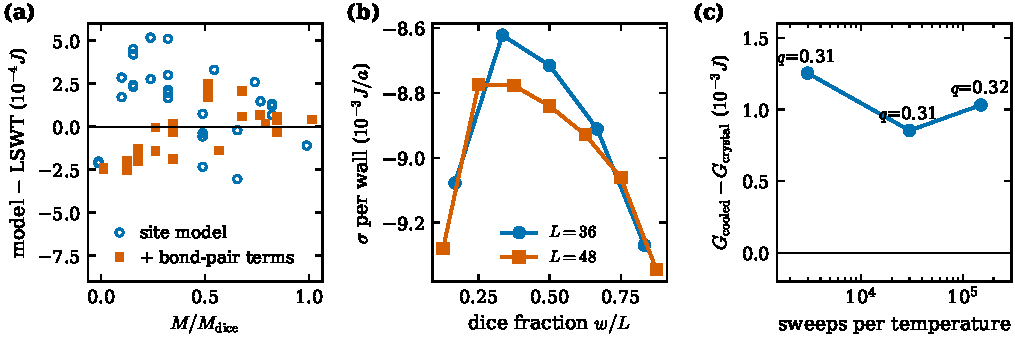
\includegraphics[width=0.94\textwidth]{figs/figA2_tests.pdf}
\caption{(a)~Out-of-sample test of Eq.~(\ref{eq:coord}) on 71 periodic crystals, relative to thermodynamic-limit LSWT: site model (circles) and site model with bond-pair terms (squares). Points are offset horizontally for clarity. (b)~LSWT energy per straight dice$|$square wall for a dice strip of width $w$ in a square background on $L=36$ and $48$ tori. The walls are $w$ and $L-w$ rows apart, and closely spaced walls ($w/L$ near 0 or 1) have lower energy. (c)~Free energy $G=e_0-hm$ of the state reached by cooling to $T=0.005J$ relative to the $\Md/2$ crystal, for three cooling rates; labels give the overlap $q$ with the crystal.}
\label{fig:A2}
\end{figure*}
%=====================================================================

\emph{Coordination model.} The training set comprises the tilt family (dice, square-type, strips of width 6 and 12, and the superlattice of alternating six-row square-type and three-row dice strips, $s6d3$) at $L=18$ and $24$, each with 0 to 600 random hexagon flips, 128 tilings in total. The site model, Eq.~(\ref{eq:coord}), gives an rms residual of $1.55\times10^{-4}J$ ($1.60\times10^{-4}J$ leave-one-out). The largest single residual is $4.1\times10^{-4}J$. Residuals averaged over each class of starting structure and over each number of flips are below $1.8\times10^{-4}J$ and show no trend with the number of flips. Adding the densities of the ten bond types $(z_i,z_j)$ reduces the rms residual to $0.82\times10^{-4}J$ ($0.87\times10^{-4}J$ leave-one-out). The out-of-sample test on 71 periodic crystals [Fig.~\ref{fig:A2}(a)] gives $2.4\times10^{-4}J$ for the site model and $1.5\times10^{-4}J$ with pair terms. Within groups of crystals that share the same $m$ and the same histogram, LSWT energies differ by up to $3.5\times10^{-4}J$ (at $\Md/3$) and $3.1\times10^{-4}J$ (at $\Md/2$). The Spearman rank correlation between the pair model and LSWT within each $m$ is $0.76$--$0.92$. For the two $\Md/2$ structures evaluated with both methods, LSWT ($-0.64945$ vs $-0.64914J$) and QMC ($\delta e=-5.3(4)$ vs $-4.8(4)\times10^{-3}J$ at $L=24$) give the same order. Two $\Md/3$ structures with the same histogram, separated by $2.5\times10^{-4}J$ in LSWT, give in QMC $-4.39(13)\times10^{-3}J$ at $L=36$ and $-3.6(3)\times10^{-3}J$ at $L=24$ (the LSWT-preferred one) and $-3.88(53)\times10^{-3}J$ at $L=18$; these values, at different sizes, do not establish the order. The best $\Md/6$ and $\Md/3$ structures of the class-resolved search lie $2.5$ and $1.1\times10^{-4}J$ below the best structures selected by histogram alone. In QMC at $L=36$ they are lower by $0.45(15)$ and $0.14(16)\times10^{-3}J$, from three and two independent runs. LSWT orderings at the level of a few $10^{-4}J$ are therefore borne out, whereas differences of order $10^{-4}J$ are not resolved by QMC.

\emph{Walls.} Straight-wall superlattices at $m=1/18$, $1/12$ and $1/9$ have LSWT energies $-0.65076$, $-0.64718$ and $-0.64246J$, compared with $-0.65281$, $-0.64945$ and $-0.64492J$ for the best crystals. Their histograms contain 6\%, 8\% and 17\% hubs, respectively.

\emph{Cooling.} Starting from the melted state at $T=0.05J$ and cooling to $0.005J$ in 19 steps with 3000, 30\,000 or 150\,000 sweeps per step ($L=24$, $h=0.19J$) always ends with $q\approx0.31$ and $G$ above the crystal by $0.9$--$1.3\times10^{-3}J$.

%=====================================================================
\section{Spin-wave hull and finite-size effects}\label{app:lswt}

\begin{figure}[t]
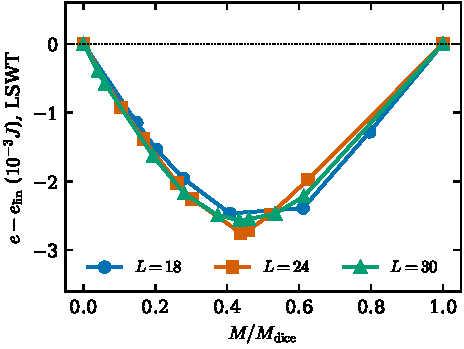
\includegraphics[width=0.9\columnwidth]{figs/figA1_lswt_L.pdf}
\caption{LSWT energies of annealed tilings relative to the square-to-dice line for $L=18$, $24$, $30$. The lower envelope is size-independent to within $3\times10^{-4}J$.}
\label{fig:A1}
\end{figure}
%=====================================================================

The LSWT energies of the annealed tilings relative to the linear interpolation are independent of system size for $L=18$--$30$ (Fig.~\ref{fig:A1}). This justifies the use of $L\le36$ tori. LSWT underestimates the QMC deviations of the crystals by factors of $1.5$, $1.4$, $1.3$, $1.22$ and $1.25$ at $\Md/6$, $\Md/3$, $\Md/2$, $\frac35\Md$ and $2\Md/3$, and the step fields above $\Md/4$ by factors of $1.2$--$1.4$. For periodic crystals with an extensive moment the LSWT energy per site on an $L=36$ torus equals the thermodynamic limit to better than $5\times10^{-6}J$; no term proportional to the total moment is present (Sec.~\ref{sec:methods}). LSWT reproduces the robust part of the hull, the $\Md/3$ and $\frac35\Md$ crystals and the jump to dice, but differences of order $10^{-4}J$ are not resolved by QMC (Appendix~\ref{app:tests}). For periodic crystals we also evaluate LSWT directly in the thermodynamic limit by Bloch diagonalization of the supercell ($6\times6$ to $64\times64$ $k$ points). For the crystals checked it agrees with $L=36$ tori to $10^{-8}J$. The $\frac35\Md$ crystal is the deepest LSWT hull point as well ($-4.29\times10^{-3}J$ in the thermodynamic limit, compared with $-3.89\times10^{-3}J$ for $\Md/2$), and LSWT underestimates its QMC deviation by a factor of $1.22$. The LSWT step fields into and out of its plateau, $0.125J$ and $0.213J$, are smaller than the QMC values by factors of $1.38$ and $1.26$.

\begin{figure}[!htbp]
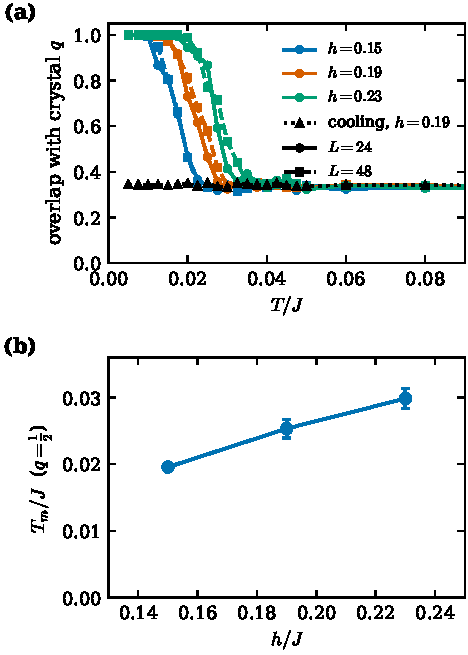
\includegraphics[width=\columnwidth]{figs/fig9_melting.pdf}
\caption{Thermal stability of the $\Md/2$ crystal (tiling Monte Carlo with the QMC-scaled coordination model, local hexagon flips, crystal tilt sector). (a)~Overlap $q$ of the tiling with the crystal on heating for three fields and two sizes, and on slow cooling from the disordered state (triangles). $q\simeq\frac13$ is the value for an uncorrelated tiling. (b)~Melting temperature, defined by $q=\frac12$.}
\label{fig:melt}
\end{figure}

%=====================================================================
\section{Finite temperature in an effective tiling model}\label{app:finiteT}

To study thermal stability we treat the tiling as a classical degree of freedom with the coordination free energy of Sec.~\ref{sec:zero}, scaled to QMC, and simulate it with local hexagon flips in the tilt sector of the crystal.
%=====================================================================



When the tiling can rearrange, for example during growth, self-assembly or in a programmable array, the plateau crystals compete with the configurational entropy of the tiling. We model this with the QMC-scaled coordination free energy and local hexagon flips in the crystal's tilt sector. We study the $\Md/2$ crystal, the deepest untilted crystal we find. The $\frac35\Md$ crystal is tilted by $30^\circ$ (Appendix~\ref{app:geom}) and lies in a different tilt sector, which local flips cannot reach. The spins are not sampled thermally. Because the coordination model depends only on the histogram and on $m$, all perfectly sorted arrangements with the histogram of the $\Md/2$ crystal are degenerate with it in this model. The overlap $q$ with one representative crystal is therefore only a proxy for crystalline order, and the pair terms of the defect lattice gas (Sec.~\ref{sec:gas}) would be needed to select a single arrangement. The temperatures below are therefore melting scales of this effective model, not transition temperatures of the full spin-plus-tiling system. Heating the $\Md/2$ crystal at fixed field [Fig.~\ref{fig:melt}(a)] produces a sharp loss of crystalline overlap at $T_m=0.020$, $0.025$ and $0.030J$ for $h=0.15$, $0.19$ and $0.23J$. The results for $L=24$ and $48$ coincide. $T_m$ increases with $h$ [Fig.~\ref{fig:melt}(b)] because the field deepens the hull minimum at $\Md/2$. In this effective model at fixed $[111]$ tilt, whose hull has only the $\Md/2$ kink, the $\Md/2$ crystal is the ground state for $h\approx0.13$--$0.25J$; all three fields lie in this window, although in the full QMC hull of Table~\ref{tab:crystals} the $\Md/2$ crystal only touches the hull. On slow cooling from the disordered state, however, the system does not recrystallize. The overlap remains at the random value and the magnetization freezes near $0.47\Md$. Cooling 50 times more slowly does not change this [Fig.~\ref{fig:A2}(c)]. The final state has $G=e_0-hm$ ($S=\frac12$) higher than the crystal by $0.9$--$1.3\times10^{-3}J$ per site. It is therefore a metastable state of the local-flip dynamics, i.e., kinetic trapping, and not evidence for an equilibrium glass phase. This trapping is a practical consideration for any realization in which the tiling is annealed.

Two omitted effects can be estimated. (i)~\emph{Magnon entropy.} From Bloch LSWT, the magnon free energy per site of the crystals at $T=0.02$--$0.03J$ is $-1.6\times10^{-6}$ (square-type) to $-7\times10^{-5}J$ (dice), roughly proportional to $m$. On melting at $h=0.19J$ the magnetization drops by $\Delta m\approx0.018$ and the configurational entropy rises by $\Delta s\approx0.1$ per site. The magnon correction shifts $T_m$ by about $\Delta F_{\rm mag}/\Delta s\sim10^{-4}J$ and the step fields by $\lesssim5\times10^{-4}J$, both negligible. (ii)~\emph{Tilt-changing moves} enlarge the configuration space of the disordered state but not of the locked crystal. They would therefore lower $T_m$, so our values are best read as upper estimates within this model. A joint treatment of spin and tiling fluctuations is left for future work.

\FloatBarrier
%=====================================================================
\begin{thebibliography}{99}

\bibitem{Villain1980} J. Villain, R. Bidaux, J.-P. Carton, and R. Conte, Order as an effect of disorder, \href{https://doi.org/10.1051/jphys:0198000410110126300}{J. Phys. (Paris) \textbf{41}, 1263 (1980)}.

\bibitem{Henley1989} C. L. Henley, Ordering due to disorder in a frustrated vector antiferromagnet, \href{https://doi.org/10.1103/PhysRevLett.62.2056}{Phys. Rev. Lett. \textbf{62}, 2056 (1989)}.

\bibitem{Henley2006} C. L. Henley, Order by disorder and gaugelike degeneracy in a quantum pyrochlore antiferromagnet, \href{https://doi.org/10.1103/PhysRevLett.96.047201}{Phys. Rev. Lett. \textbf{96}, 047201 (2006)}.

\bibitem{Sutherland1986} B. Sutherland, Localization of electronic wave functions due to local topology, \href{https://doi.org/10.1103/PhysRevB.34.5208}{Phys. Rev. B \textbf{34}, 5208 (1986)}.

\bibitem{Vidal1998} J. Vidal, R. Mosseri, and B. Dou\c{c}ot, Aharonov-Bohm cages in two-dimensional structures, \href{https://doi.org/10.1103/PhysRevLett.81.5888}{Phys. Rev. Lett. \textbf{81}, 5888 (1998)}.

\bibitem{LiebMattis1962} E. Lieb and D. Mattis, Ordering energy levels of interacting spin systems, \href{https://doi.org/10.1063/1.1724276}{J. Math. Phys. \textbf{3}, 749 (1962)}.

\bibitem{Lieb1989} E. H. Lieb, Two theorems on the Hubbard model, \href{https://doi.org/10.1103/PhysRevLett.62.1201}{Phys. Rev. Lett. \textbf{62}, 1201 (1989)}.

\bibitem{Wessel2003} S. Wessel, A. Jagannathan, and S. Haas, Quantum antiferromagnetism in quasicrystals, \href{https://doi.org/10.1103/PhysRevLett.90.177205}{Phys. Rev. Lett. \textbf{90}, 177205 (2003)}.

\bibitem{Jagannathan2006} A. Jagannathan, R. Moessner, and S. Wessel, Inhomogeneous quantum antiferromagnetism on periodic lattices, \href{https://doi.org/10.1103/PhysRevB.74.184410}{Phys. Rev. B \textbf{74}, 184410 (2006)}.

\bibitem{Szallas2009} A. Szallas, A. Jagannathan, and S. Wessel, Phason-disordered two-dimensional quantum antiferromagnets, \href{https://doi.org/10.1103/PhysRevB.79.172406}{Phys. Rev. B \textbf{79}, 172406 (2009)}.

\bibitem{Jagannathan2012} A. Jagannathan, B. Dou\c{c}ot, A. Szallas, and S. Wessel, Geometric fluctuations in a two-dimensional quantum antiferromagnet, \href{https://doi.org/10.1103/PhysRevB.85.094434}{Phys. Rev. B \textbf{85}, 094434 (2012)}.

\bibitem{Jagannathan2013} A. Jagannathan and A. Szallas, Geometry fluctuations and Casimir effect in a quantum antiferromagnet, \href{https://doi.org/10.1140/epjb/e2012-31033-y}{Eur. Phys. J. B \textbf{86}, 76 (2013)}.

\bibitem{BloteHilhorst1982} H. W. J. Bl\"ote and H. J. Hilhorst, Roughening transitions and the zero-temperature triangular Ising antiferromagnet, \href{https://doi.org/10.1088/0305-4470/15/11/011}{J. Phys. A \textbf{15}, L631 (1982)}.

\bibitem{Kenyon2006} R. Kenyon, A. Okounkov, and S. Sheffield, Dimers and amoebae, \href{https://doi.org/10.4007/annals.2006.163.1019}{Ann. Math. \textbf{163}, 1019 (2006)}.

\bibitem{Sandvik1999} A. W. Sandvik, Stochastic series expansion method with operator-loop update, \href{https://doi.org/10.1103/PhysRevB.59.R14157}{Phys. Rev. B \textbf{59}, R14157 (1999)}.

\bibitem{Syljuasen2002} O. F. Sylju\aa sen and A. W. Sandvik, Quantum Monte Carlo with directed loops, \href{https://doi.org/10.1103/PhysRevE.66.046701}{Phys. Rev. E \textbf{66}, 046701 (2002)}.

\bibitem{Sandvik1997} A. W. Sandvik, Finite-size scaling of the ground-state parameters of the two-dimensional Heisenberg model, \href{https://doi.org/10.1103/PhysRevB.56.11678}{Phys. Rev. B \textbf{56}, 11678 (1997)}.

\bibitem{Colpa1978} J. H. P. Colpa, Diagonalization of the quadratic boson Hamiltonian, \href{https://doi.org/10.1016/0378-4371(78)90160-7}{Physica A \textbf{93}, 327 (1978)}.

\bibitem{WatanabeBrauner2011} H. Watanabe and T. Brauner, Number of Nambu-Goldstone bosons and its relation to charge densities, \href{https://doi.org/10.1103/PhysRevD.84.125013}{Phys. Rev. D \textbf{84}, 125013 (2011)}.

\bibitem{Watanabe2012} H. Watanabe and H. Murayama, Unified description of Nambu-Goldstone bosons without Lorentz invariance, \href{https://doi.org/10.1103/PhysRevLett.108.251602}{Phys. Rev. Lett. \textbf{108}, 251602 (2012)}.

\bibitem{Hidaka2013} Y. Hidaka, Counting rule for Nambu-Goldstone modes in nonrelativistic systems, \href{https://doi.org/10.1103/PhysRevLett.110.091601}{Phys. Rev. Lett. \textbf{110}, 091601 (2013)}.

\bibitem{Rokhsar1988} D. S. Rokhsar and S. A. Kivelson, Superconductivity and the quantum hard-core dimer gas, \href{https://doi.org/10.1103/PhysRevLett.61.2376}{Phys. Rev. Lett. \textbf{61}, 2376 (1988)}.

\bibitem{Moessner2001} R. Moessner and S. L. Sondhi, Resonating valence bond phase in the triangular lattice quantum dimer model, \href{https://doi.org/10.1103/PhysRevLett.86.1881}{Phys. Rev. Lett. \textbf{86}, 1881 (2001)}.

\bibitem{MoessnerSondhiChandra2001} R. Moessner, S. L. Sondhi, and P. Chandra, Phase diagram of the hexagonal lattice quantum dimer model, \href{https://doi.org/10.1103/PhysRevB.64.144416}{Phys. Rev. B \textbf{64}, 144416 (2001)}.

\bibitem{Bak1982} P. Bak and R. Bruinsma, One-dimensional Ising model and the complete devil's staircase, \href{https://doi.org/10.1103/PhysRevLett.49.249}{Phys. Rev. Lett. \textbf{49}, 249 (1982)}.

\bibitem{Kageyama1999} H. Kageyama \textit{et al.}, Exact dimer ground state and quantized magnetization plateaus in the two-dimensional spin system SrCu$_2$(BO$_3$)$_2$, \href{https://doi.org/10.1103/PhysRevLett.82.3168}{Phys. Rev. Lett. \textbf{82}, 3168 (1999)}.

\bibitem{Honecker2004} A. Honecker, J. Schulenburg, and J. Richter, Magnetization plateaus in frustrated antiferromagnetic quantum spin models, \href{https://doi.org/10.1088/0953-8984/16/11/025}{J. Phys.: Condens. Matter \textbf{16}, S749 (2004)}.

\bibitem{PencShannonShiba2004} K. Penc, N. Shannon, and H. Shiba, Half-magnetization plateau stabilized by structural distortion in the antiferromagnetic Heisenberg model on a pyrochlore lattice, \href{https://doi.org/10.1103/PhysRevLett.93.197203}{Phys. Rev. Lett. \textbf{93}, 197203 (2004)}.

\bibitem{Mishra2020} S. Mishra \textit{et al.}, Topological frustration induces unconventional magnetism in a nanographene, \href{https://doi.org/10.1038/s41565-019-0577-9}{Nat. Nanotechnol. \textbf{15}, 22 (2020)}.

\bibitem{Mishra2021} S. Mishra \textit{et al.}, Observation of fractional edge excitations in nanographene spin chains, \href{https://doi.org/10.1038/s41586-021-03842-3}{Nature \textbf{598}, 287 (2021)}.

\bibitem{Khajetoorians2019} A. A. Khajetoorians, D. Wegner, A. F. Otte, and I. Swart, Creating designer quantum states of matter atom-by-atom, \href{https://doi.org/10.1038/s42254-019-0108-5}{Nat. Rev. Phys. \textbf{1}, 703 (2019)}.

\bibitem{Scholl2021} P. Scholl \textit{et al.}, Quantum simulation of 2D antiferromagnets with hundreds of Rydberg atoms, \href{https://doi.org/10.1038/s41586-021-03585-1}{Nature \textbf{595}, 233 (2021)}.

\bibitem{WangSandvik2006} L. Wang and A. W. Sandvik, Low-energy dynamics of the two-dimensional $S=1/2$ Heisenberg antiferromagnet on percolating clusters, \href{https://doi.org/10.1103/PhysRevLett.97.117204}{Phys. Rev. Lett. \textbf{97}, 117204 (2006)}.

\bibitem{DataRepo} S. Yoo \textit{et al.}, code and data for this article (2026), \url{https://github.com/cywon-commits/lozenge-quantum-tiling}.

\end{thebibliography}

\end{document}
